\chapter{Calorimeter commissioning}
\label{ch:commissioning}

The commissioning of the SuperNEMO demonstrator has begun in $2019$ and calibration acquisitions were taken and analysed by the collaboration.

The first two sections describe the start-up of the calorimeter, with the first data acquisitions and the various calibration operations carried out by the collaboration.
Studies led to characterise the waveform baseline and pulse shape are presented.
Optical modules have are aligned in gain and a general procedure for their energy calibration is given.

The rest of the chapter deals with the work done within the framework of this PhD in order to verify the operating state of the calorimeter and its signal cables, after integration.
All cable lengths are measured by an innovative technique, and the corresponding time offset of each electronic channel is characterised.
An additional time offset brought by the electronic boards is also measured.

\section{Optical modules calibration}

It is necessary to check the correct operation of the whole calorimeter as well as each individual optical module, in order to repair and correct it if necessary.

\subsection{Pulse shape studies}
\label{subsec:SN_pulse_shape}

It is interesting to study the shape of the pulses sampled by the electronic boards, as it allows the identification of the presence of pre- or post-pulses.
This may be caused by undesired interactions, such as contamination of photomultipliers' vacuum by Helium, or the interaction of photons from the laboratory lighting, due to defects in the detector's light tightness.
A study performed by William Queen, a PhD student at UCL, allowed to determine a reference model for the expected shape of calorimeter waveforms.
An example of an awaited waveform is given in fig.~\ref{fig:waveform}.
The pulses received by the calorimeter can then be compared with this standard waveform, allowing any issues to be detected and resolved.
\begin{figure}[h!]
  \centering
  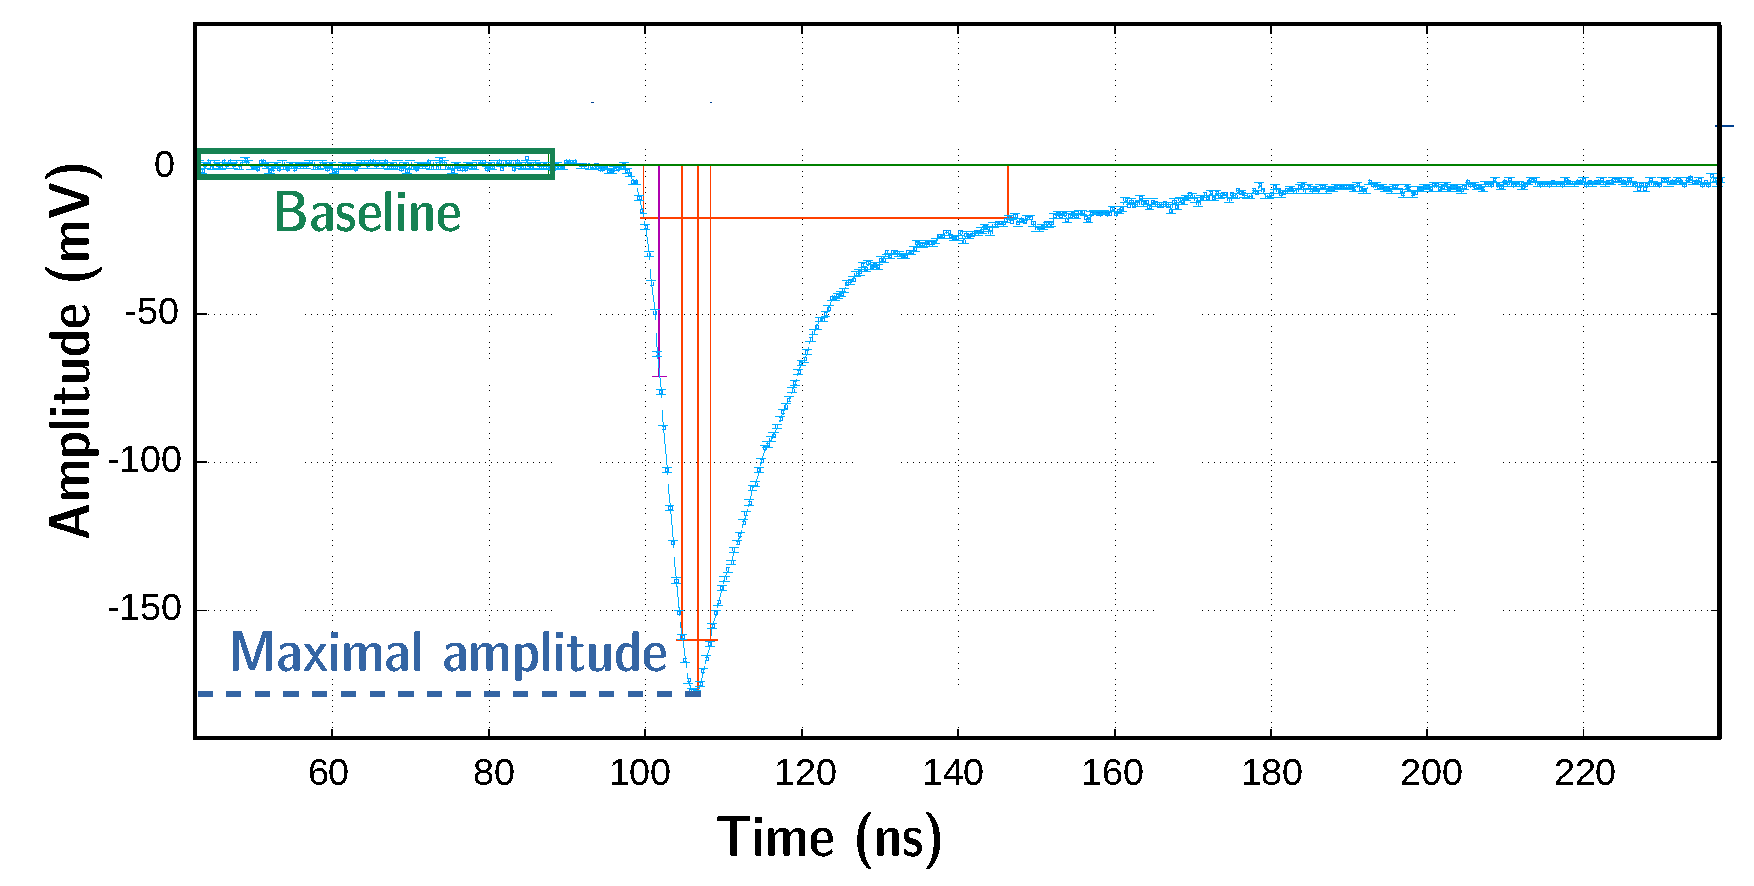
\includegraphics[width=1\textwidth]{commissioning/fig_commissioning/waveform.pdf}
  \caption{Calorimeter waveform visualisation with the SNFee software.
    \label{fig:waveform}}
\end{figure}



\subsection{Baseline studies}

The baseline is the part of the signal located before the signal rising edge.
Slight signal fluctuations can be observed in this area due to electronic noise, for example.
By averaging the amplitude value in this area, a reference can be defined to calculate the pulse amplitude.
This average is calculated by default directly by the calorimeter front-end boards, over the first $6.25$ nanoseconds of the signal.
In order to minimise the impact of statistical fluctuations on the baseline calculation, a more efficient analysis has been developed by Hichem Tedjditi, a PhD student at the CPPM, allowing to calculate it over an extended time.
The calculation of this average starts at the opening of the acquisition window, up to the rising edge of the signal pulse, which is detected automatically.
The presence of pre-pulses is also automatically characterised.
This analysis is done off-line and participates in the verification of the optical modules condition, after the installation of the calorimeter, and throughout the data acquisition of the demonstrator.

\subsection{Gain studies}


When a particle deposits energy as it interacts in the scintillator, the detection chain that follows enables a quantity of charge to be recovered at the PM voltage divider, that is proportional to the first energy deposited and depends on the high voltage applied to the photomultiplier.
In the SuperNEMO detector, these voltages can be adjusted individually for each block.
Charge and amplitude spectra can be obtained for each optical module and therefore depend on the high voltage applied.
As the optical modules are triggered by a signal amplitude threshold, it is necessary that the gains of all the optical modules of the calorimeter are equalised, in order to have comparable threshold values.
For the SuperNEMO calorimeter, this value has been set at an amplitude of $200$~mV for $1$~MeV deposited.
Each optical module has then to be calibrated after installation, in order to reach this standard value and equalise all the PM responses.
The current study has been led by Axel Pin, a PhD student from CENBG.

This calibration consists in the optical module gains alignment, by obtaining a new high voltage value to be applied.
To determine the current gain of an optical module, one must first obtain its amplitude (or charge) spectrum and then locate a particular point on this spectrum.
For this study, the chosen point is located at the end of the spectrum, where the only contribution of \Tl\ is expected.
To obtain these spectra with a reasonably large statistics, long runs (few hours) have been taken with the demonstrator, without the $^{207}$Bi calibration sources.
Once this gain is obtained, a reference gain is computed using simulations of \Tl\ decays.
The same particular point is determined, which corresponds to a given energy, as simulations allow to construct energy spectra.
Therefore, two gains are obtained one for real data and the other for simulations, allowing to determine the optimal high voltage value to apply for each photomultiplier.
The gains distributions before and after equalisation are presented in Fig.~\ref{fig:Axel_gain}.
The gain adjustment method have been effective as the distribution mean stands at $606.5\pm1.4$~mV at $3$~MeV, considering a $8$~\% FWHM at $1$~MeV, for the $440$ $8$~inches photomultipliers.
\begin{figure}[h!]
  \centering
  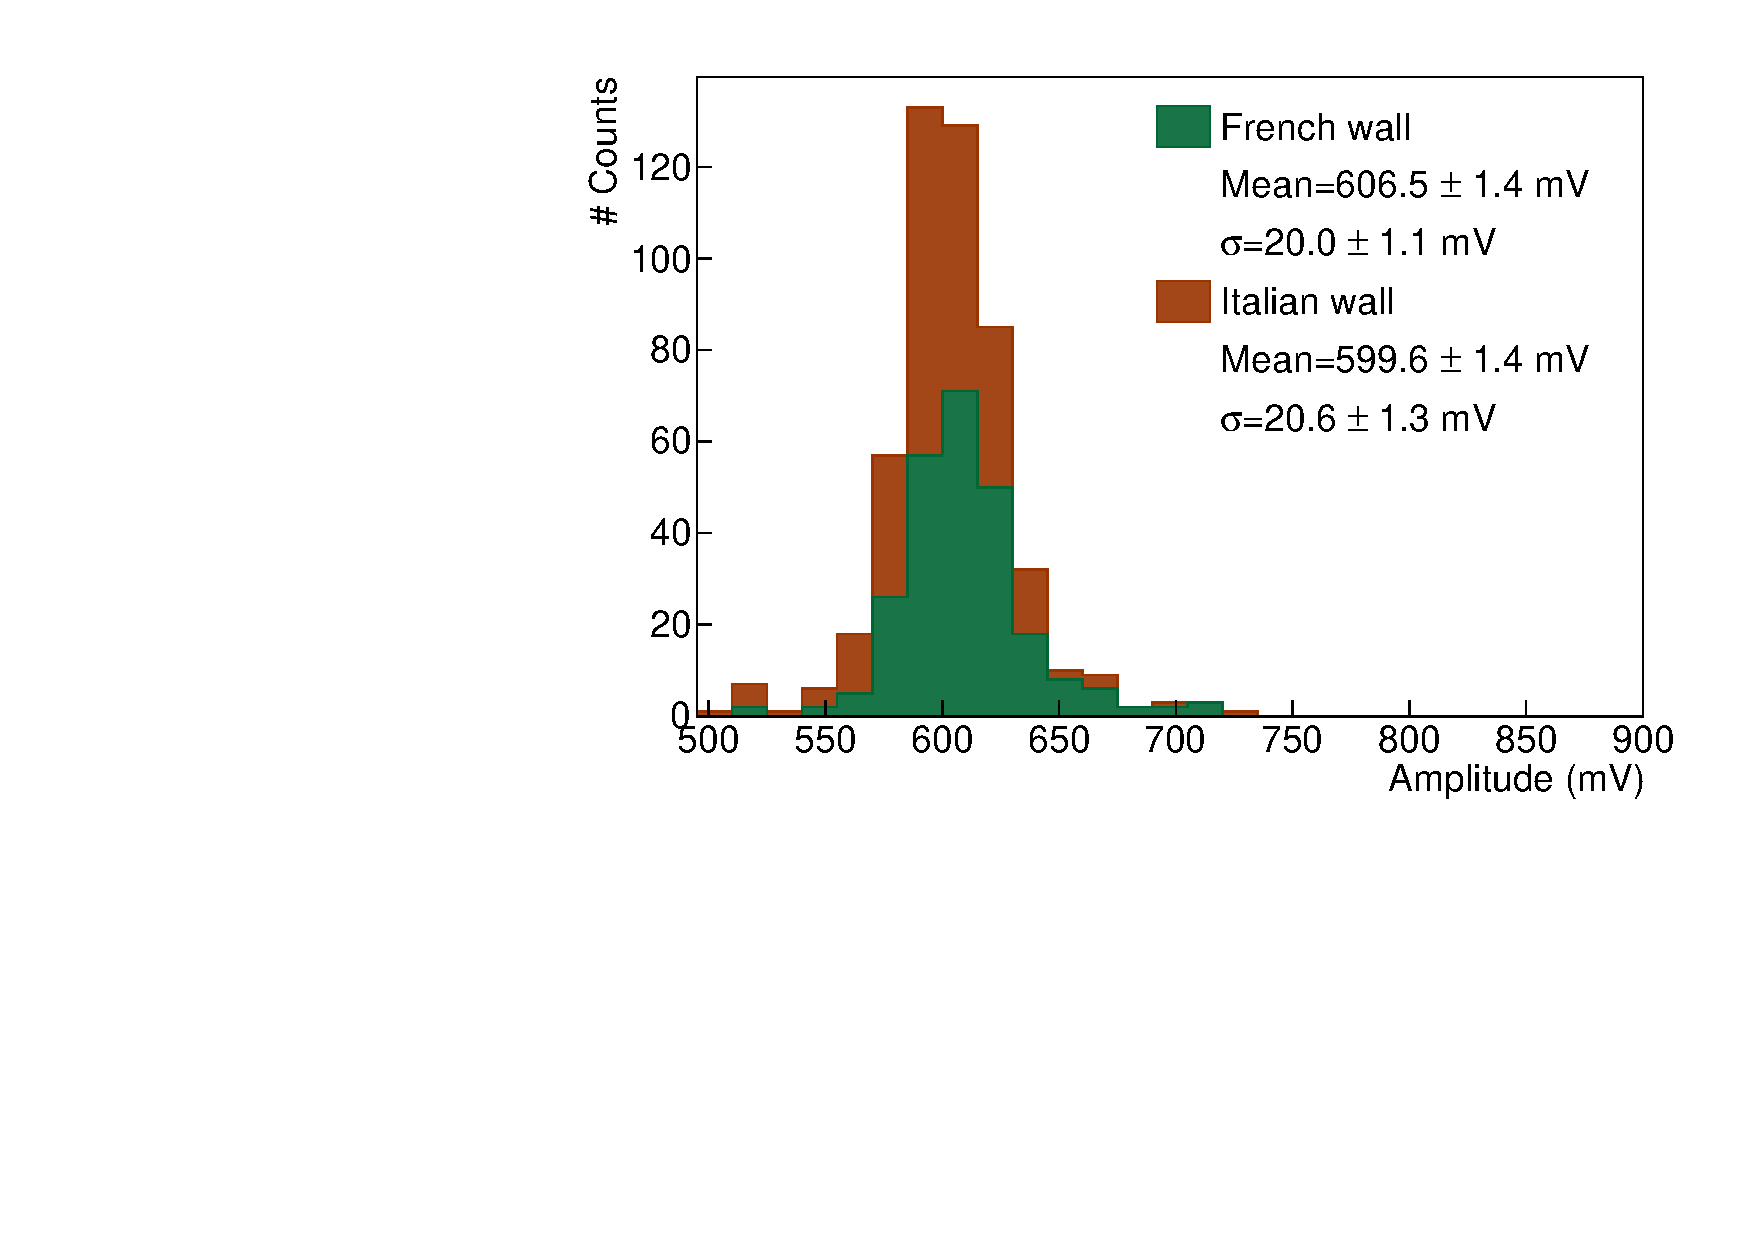
\includegraphics[width=0.8\textwidth]{commissioning/fig_commissioning/equal_gains_Axel.pdf}
  \caption{Amplitude spectra for French and Italian main wall after gain equalisation.
    \label{fig:Axel_gain}}
\end{figure}

Now the optimal high voltages have been determined for each optical module, the collaboration will have to monitor their gain, in order to insure the stability of the SuperNEMO calorimeter over time.

%% Depending on the value of this voltage, the gain $G_{OM}$ expected for a given optical module vary as:
%% \begin{equation}
%% G_{OM}=KV^{N\alpha}\,,
%% \end{equation}
%% where $K$ is a proportionality constant, $V$ is the high voltage applied to the photomultiplier, $N$ the number of dynodes and $\alpha$ is a coefficient depending on the PM characteristics.


\subsection{Energy calibration}
\label{sec:comm_energy_calibration}

As described in Sec.~\ref{subsec:OMtimeResponse}, the collected charge at photomultiplier voltage divider is proportional to the amount of incident photoelectrons, thus to the initially deposited energy inside the scintillator.
Once optical modules were assembled (optical coupling, packing, shielding integration), they were individually tested at Bordeaux laboratory, CENBG, with an electron spectrometer~\cite{HuberThesis}.
Their energy resolutions for $1$ MeV-electrons at the centre of scintillator front face were determined.
For optical modules assembled with $8$~inches photomultipliers, this value is on average of $8.19$\%.
Supply high voltages were characterised and set individually for each optical module to their to optimal values.

However, after the calorimeter integration, due to possible modifications of optical module characteristics, amplitude spectra of each optical block have to be re-aligned.
This work was also performed by Axel Pin, PhD student at CENBG.
The energy calibration method consists to find a particular point of a charge or amplitude spectrum, the Compton edge of \Tl\ for this study.
Looking for the same location on simulated \Tl\ energy spectra, a charge-energy or amplitude-energy correspondence can be made and applied to calibrate each optical module in energy.
I also performed another energy calibration using the data acquisition and simulations with a \Co\ source, using the \Co\ peak at $1$~MeV.
This is discussed in Chapter~\ref{ch:Cobalt_study}.


\section{Light Injection System}
\label{sec:LI}

The LIS is a calibration method sending light pulses in optical modules for energy calibration purposes.
It has been detailed in Chapter~\ref{ch:detector}.
In the framework of this PhD, I took part in the analysis of the first commissioning data of this system.
All results presented in this sub-section are currently being improved by the collaboration.

In Fig.~\ref{fig:LI_counts} is displayed the light intensity received by each optical module of the French main wall, for a data acquisition of $\sim20$~minutes.
Optical modules on the same main wall are divided into $5$ distinct groups, each illuminated via optical fibers by the light of one LED.
In the figure each of the $5$ area is represented.
Optical modules from area $1$ do not receive light from their associated LED, denoting a possible connection problem at the bundle (all fibers coming from one LED are grouped together in one bundle before being distributed on the calorimeter wall), or an issue with the LED itself.
It has been determined that this issue is intermittent, and sometimes affect other areas, possibly showing a more general problem related to the power supply of the LEDs.
This issue does not seem to be serious and is currently under investigation.
\begin{figure}[h!]
  \centering
  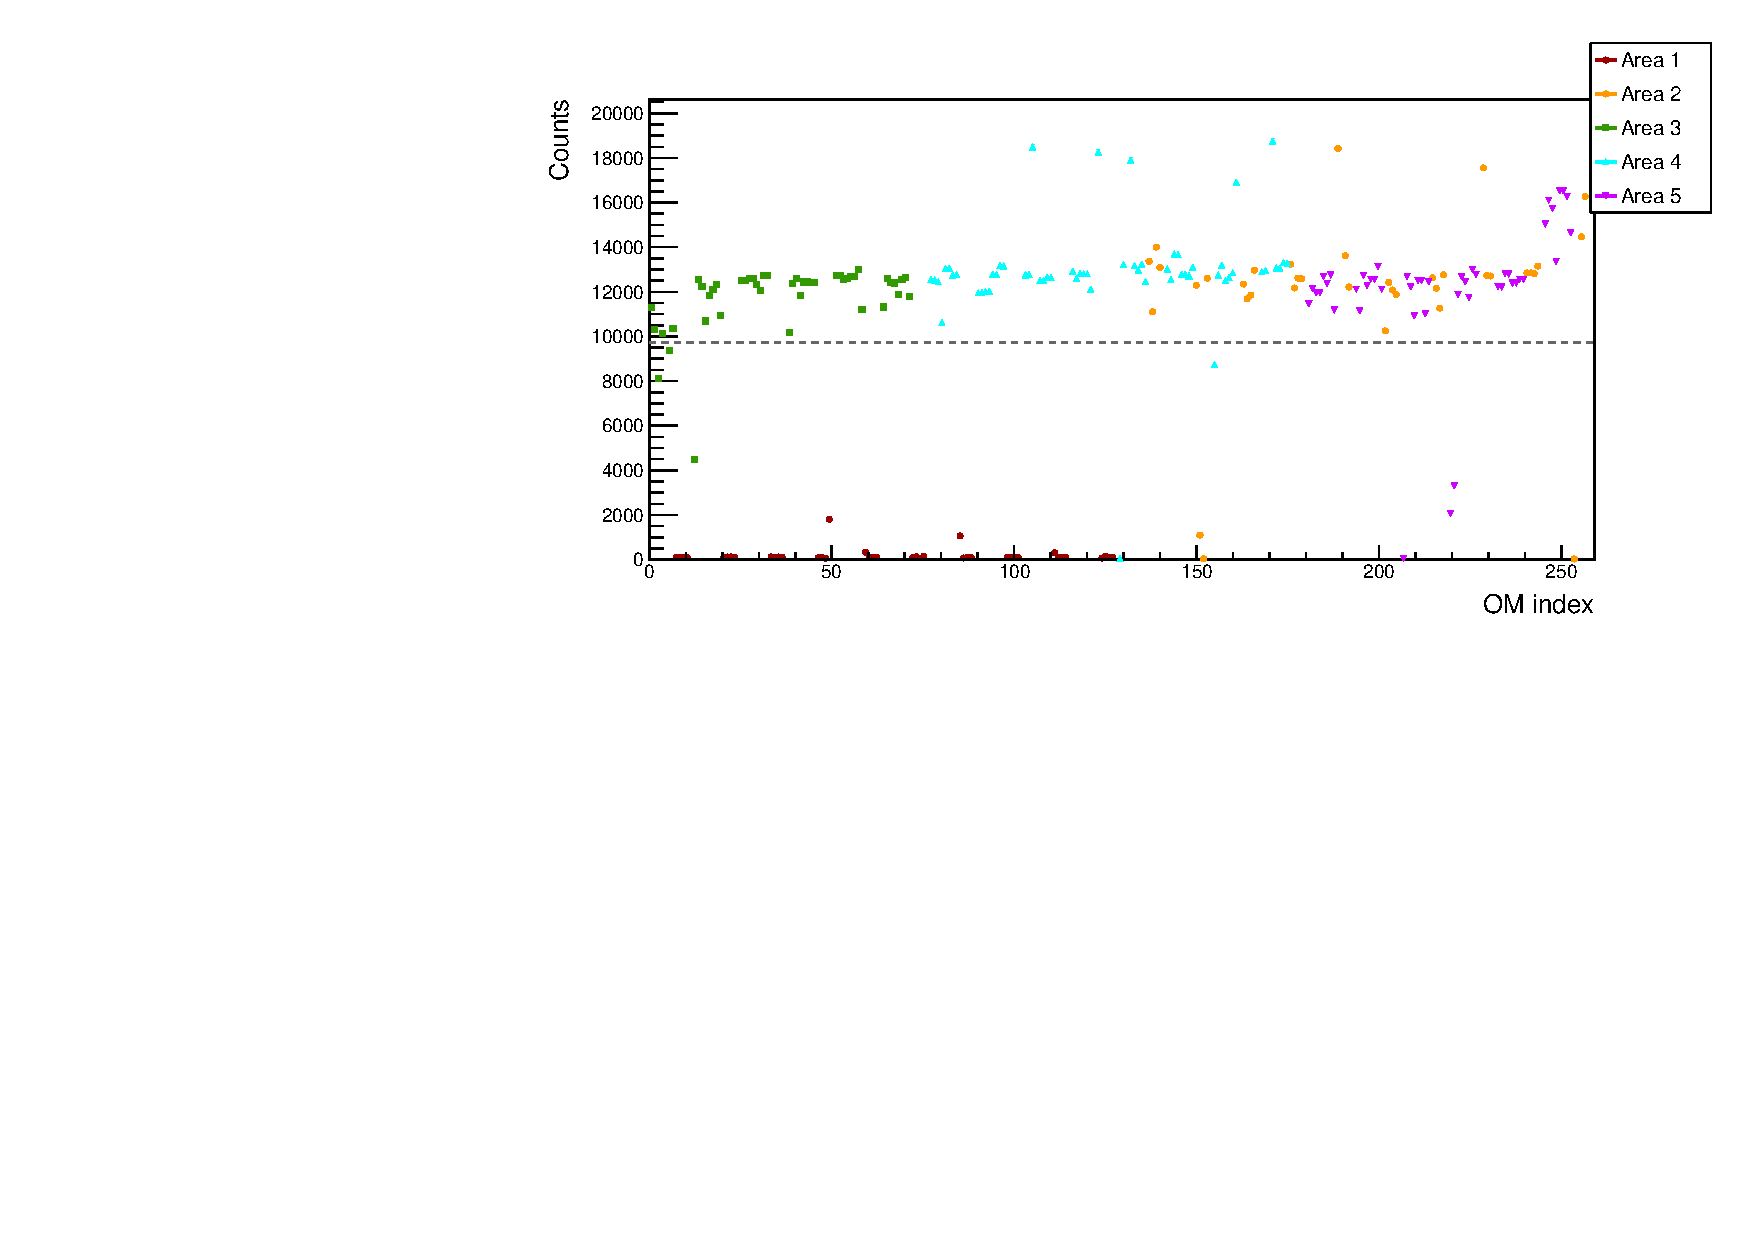
\includegraphics[width=15cm]{commissioning/fig_commissioning/LI_1d_counts.pdf}
  \caption{Quantity of light received by each OM (labelled with OM index) of the French main wall.
    Each coloured marker represents counting rates for one area of the detector, that is to say one group of optical modules lighted by the same LED.
    The area $1$ (dark red dots) is not receiving light from its corresponding LED.
    \label{fig:LI_counts}}
\end{figure}

After checking the LED operation and quantity of light received, the amplitude spectra for each area have been studied and are presented in Fig.~\ref{fig:LI_ampl}.
These spectra are very discontinuous and above all very spread out in amplitude.
The fact that the distributions are wide is not surprising, as the amount of light received by an optical module depends on many parameters, such as the location of the optical fibre in the bundle, which determines how close the fibre is to the LED.
The angle at which the optical fibre enters the scintillator can also greatly influence this quantity.
But the potentially worrying thing is that the amplitudes can go up to very high values.
In practice, the acquisition does not record signal amplitudes above a few hundred mV.
When the amplitude is even slightly too high, the signal is simply truncated.
It is then the SNFee off-line analysis software which, when trying to determine the location of the waveform peak, performs an extrapolation and gives such saturated amplitudes.
So even if these values do not correspond to the actual amount of light received by the optical modules, the amplitude is still too high compared to what is expected.
Calibration operations are underway to harmonise this quantity.
\begin{figure}[h!]
  \centering
  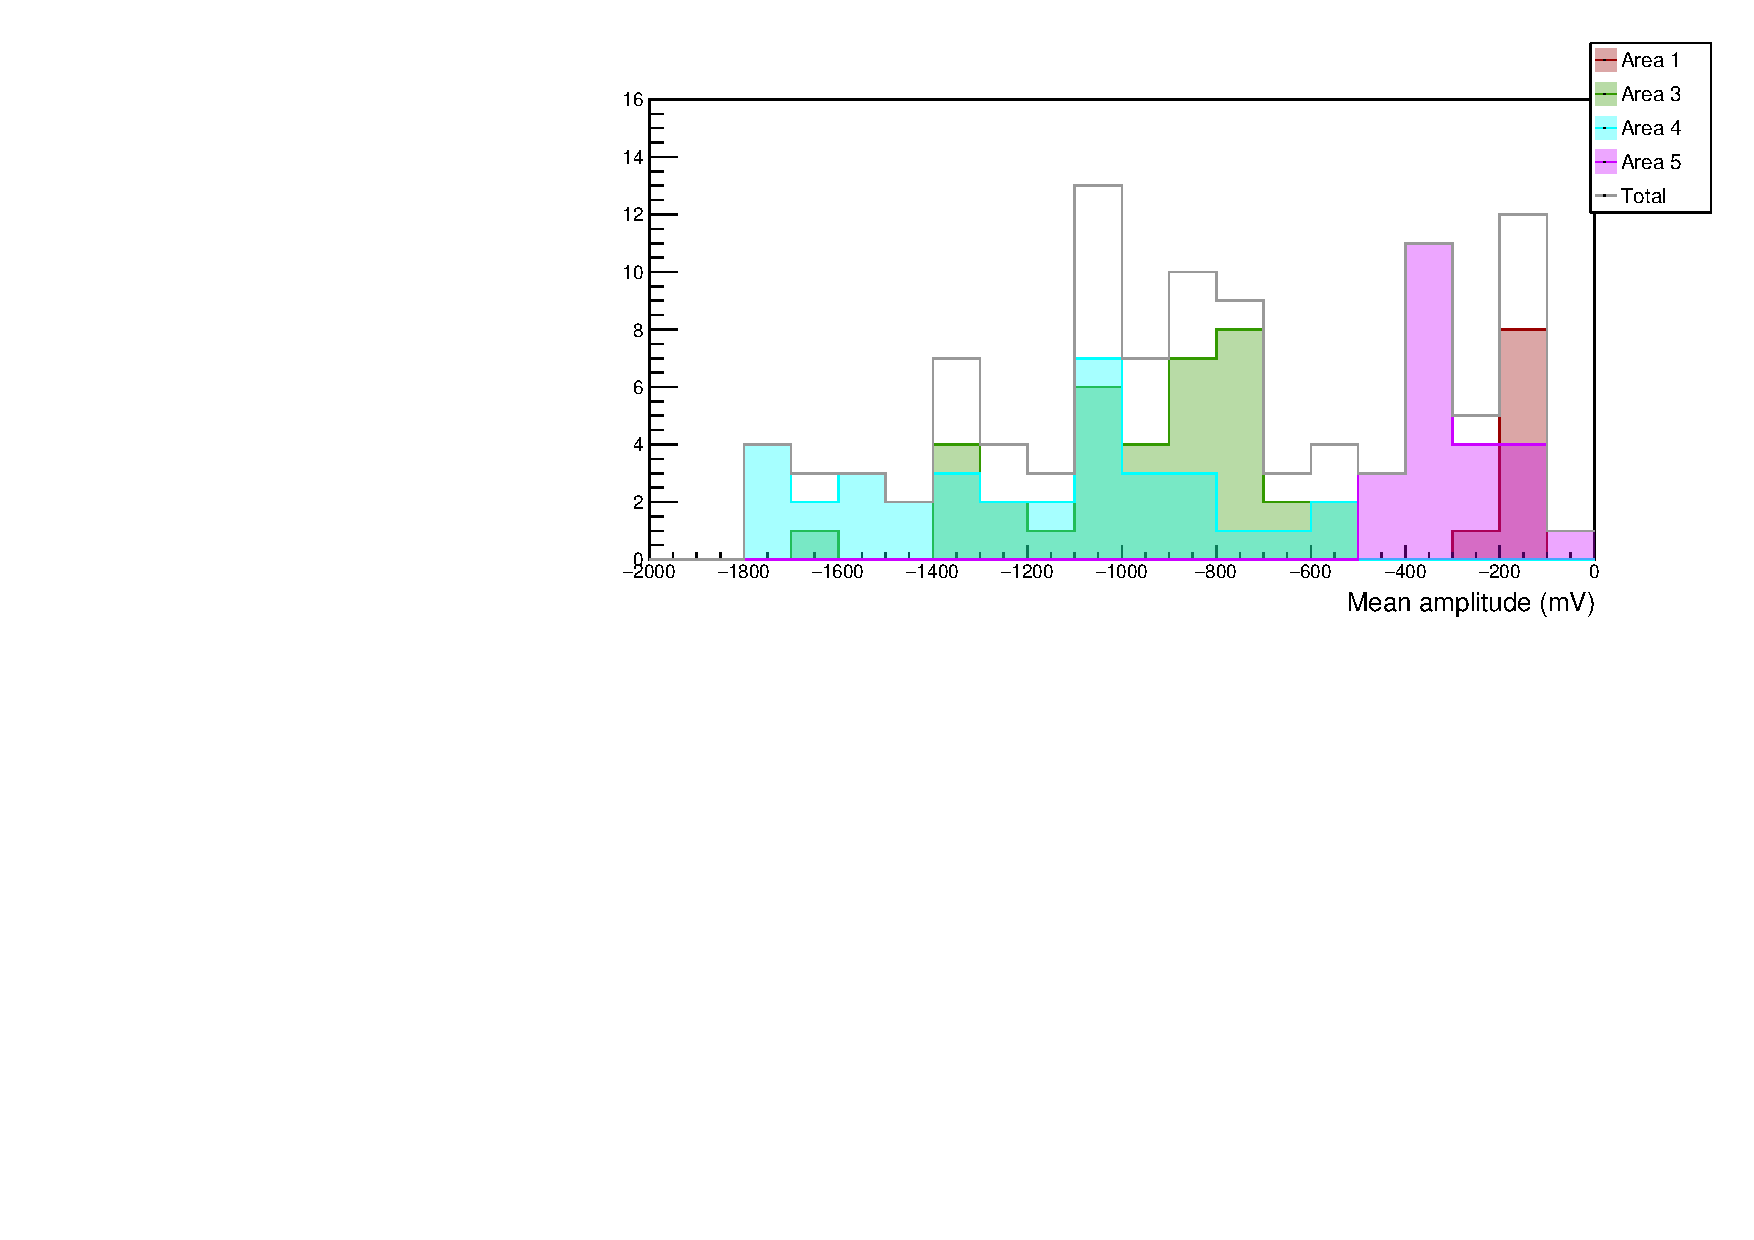
\includegraphics[width=15cm]{commissioning/fig_commissioning/LI_mean_ampl.pdf}
  \caption{The mean signal amplitude distribution for each optical module is presented.
    One colour represents one area of the French main wall.
    In Grey is the total mean amplitude distribution.
    \label{fig:LI_ampl}}
\end{figure}

In the following, the work achieved on the calorimeter commissioning, especially on timing performances, is discussed.


\section{Calorimeter cabling network}
\label{sec:reflecto}

In this section is presented an analysis performed in order to check the status of the calorimeter signal cables installed at Modane.
I was involved in most of the stages of the detector cabling, from cutting the calorimeter HV and signal cables at LAL, to their installation in Modane on the various walls of the calorimeter, via their welding to the PM voltage dividers and their organisation on the patch panel.
Although not covered in this analysis, I was also involved in the connection (under the detector) of the tracker cables and their routing from the detector to the electronics.
These steps were crucial and gave me a good knowledge of the detector I am working on.

\subsection{Motivations}

The cabling network of SuperNEMO is described in detail in Chapter~\ref{ch:detector}.
In particular, the calorimeter is segmented in $712$ optical modules, each connected to the electronics by the photomultiplier divider through $2$ cables.
The first one provides the high voltage (HV) necessary for its operation.
The other one, the so-called signal cable, is a coaxial cable collecting and transporting the charge corresponding to the optical module signal.
Regarding only the last category, $1424$ coaxial cables were cut, assembled, connector-mounted, transported and installed at LSM.

Each coaxial cable length was determined by taking into account the demonstrator design.
All external coaxial cables were designed to be $7$ meters-long -- the distance between electronic boards and patch panel being the same for all channels -- and internal cable lengths have been adapted to fit the distance from the patch panel to each optical module.
Cutting and labelling all cables lasted several weeks.
After all cables were transported and installed at LSM, we have to check each coaxial cable condition, for several reasons:
\begin{itemize*}
\item making sure that cables have not been damaged during the transport and the installation,
\item controlling if no swap between signal channels has been made during cable labelling or calorimeter cabling,
\item checking if the coaxial cables were cut at right lengths,
\item estimating time delays induced by the signal transit time inside the coaxial cables.
\end{itemize*}
The last point is essential: knowing that the  electron velocity in a coaxial cable is a determined constant value, the longer the cable, the longer it takes for the signal to reach the electronics.
As coaxial cables have different lengths, each calorimeter signal channel is characterised by a delay degrading the calorimeter time-of-flight resolution.
Therefore, each coaxial cable length has to be precisely characterised, and the transit time has to be stored in a database made available to the collaboration.

\subsection{Experimental setup}

In order to control each cable status, we used a feature provided by the SuperNEMO's electronics, where an electrical signal, called \emph{primary} pulse, is generated by the calorimeter front-end boards and sent independently to each channel.
The electric signal reflects when it encounters a high impedance, and travels back to the electronics where it is recorded, after a more or less long cable distance.
This back signal is naturally called \emph{secondary} pulse.
The Fig.~\ref{fig:reflecto_scheme} summarises the three most probable scenarios when such a pulse is sent in the SuperNEMO calorimeter cables.
\begin{itemize}
\item Fig.~\ref{subfig:reflecto_normal}: under normal cable operating conditions, the pulse travels along the coaxial cable until it reaches the photomultiplier and reflects on the divider.
\item Fig.~\ref{subfig:reflecto_pmt}: it may happen a cable is not (or badly) connected to the PM divider.
  In that case the signal reflects at the end of the internal cable.
  In this scenario, the time it took for the signal to travel this distance is the same as in the first case, but since the impedance is different, the amplitude and shape of the reflected pulse are also different.
  This scenario is addressed in Sec.~\ref{subsec:pulse_shape}.
\item Fig.~\ref{subfig:reflecto_pp}: if the cable is not connected at the patch panel level, the signal undergoes a reflection at the end of the external cable.
  This scenario is addressed in Sec.~\ref{subsec:timing}.
\end{itemize}
\begin{figure}[h!]
  \centering
  \begin{subfigure}[b]{0.3\textwidth}
    \centering
    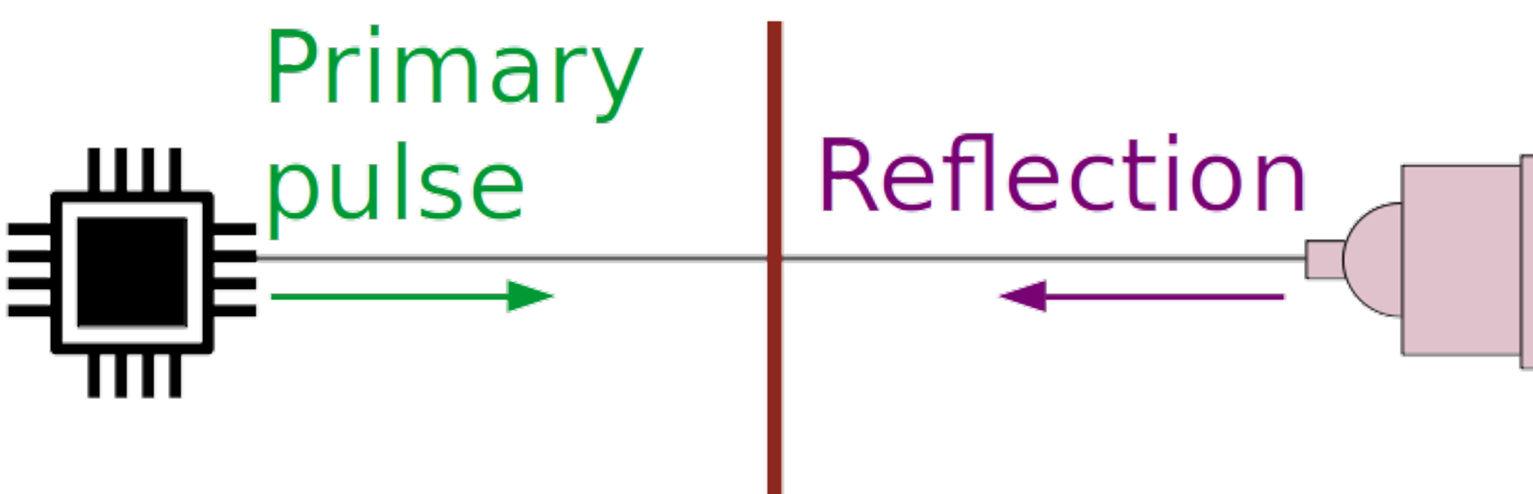
\includegraphics[width=1.1\textwidth]{commissioning/fig_commissioning/scheme_reflecto.pdf}
    \captionsetup{justification=centering}
    \caption{Normal reflection at PM divider.
      \label{subfig:reflecto_normal}}
  \end{subfigure}
  \hfill
  \begin{subfigure}[b]{0.3\textwidth}
    \centering
    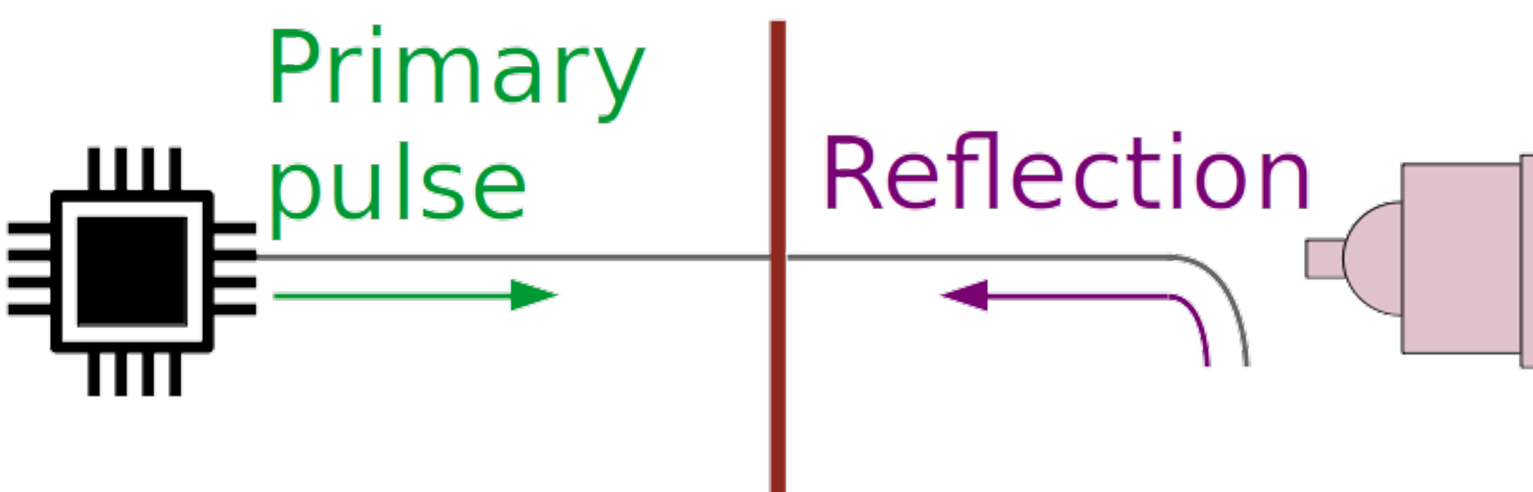
\includegraphics[width=1.1\textwidth]{commissioning/fig_commissioning/scheme_reflecto_1.pdf}
    \captionsetup{justification=centering}
    \caption{Cable not connected at PM.
      \label{subfig:reflecto_pmt}}
  \end{subfigure}
  \hfill
  \begin{subfigure}[b]{0.3\textwidth}
    \centering
    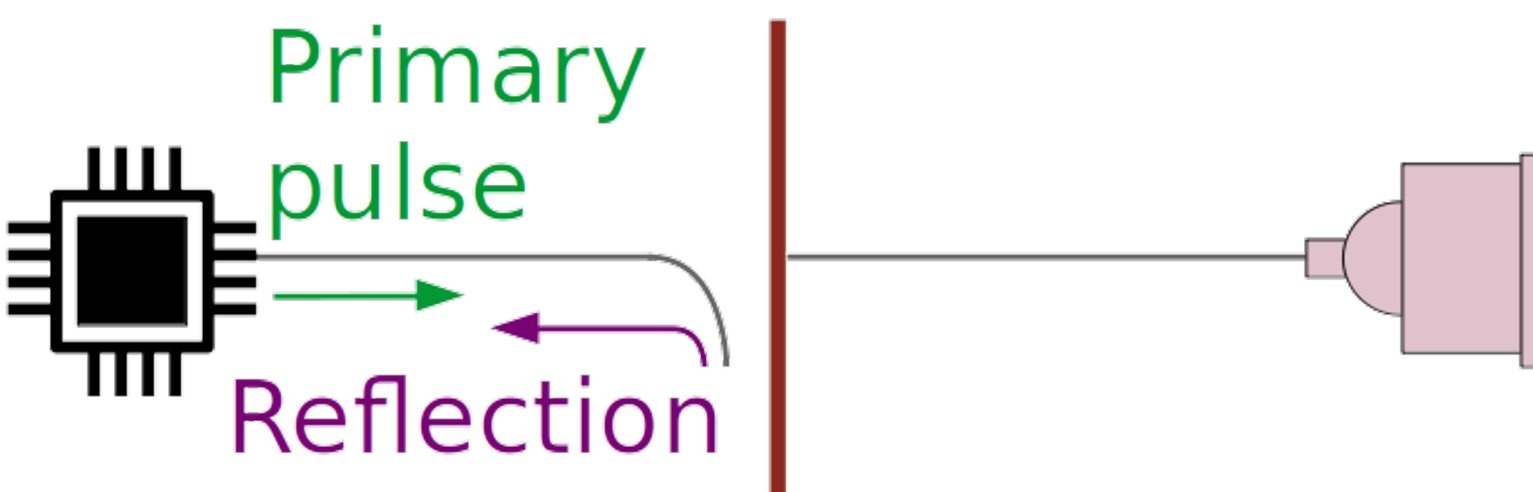
\includegraphics[width=1.1\textwidth]{commissioning/fig_commissioning/scheme_reflecto_2.pdf}
    \captionsetup{justification=centering}
    \caption{Cable not connected at the patch panel.
      \label{subfig:reflecto_pp}}
  \end{subfigure}
  \caption{Three possible scenarios occurring when a signal is sent in the SuperNEMO coaxial cables.
    The electronic boards are symbolised by black chips, and the patch panel by red vertical bars.
    The coaxial cable, pictured by horizontal lines, connects the electronics to the PM divider.
    (a) The cable is well connected at the patch panel and at the PM. The signal reflects at the PM divider.
    (b) The cable is not connected (or badly connected) at the PM divider. The signal is reflected at the end of the internal cable.
    (c) The cable is not connected (or badly connected) at the patch panel. The signal is reflected at the end of the external cable.
    \label{fig:reflecto_scheme}}
\end{figure}

An example of a set of primary and secondary pulses, under normal cable operating conditions, for $8$ inches PMs, is displayed in Fig.~\ref{fig:total_waveform}.
All primary pulses are sent almost simultaneously inside different electronic channels, so they appear all superimposed.
Depending on the cable length they travelled through, secondary pulses return to the electronics with more or less delay.
Secondary pulses are deformed by their passage through the cable, which acts as a transfer function on the signal.
\begin{figure}[h!]
  \centering
  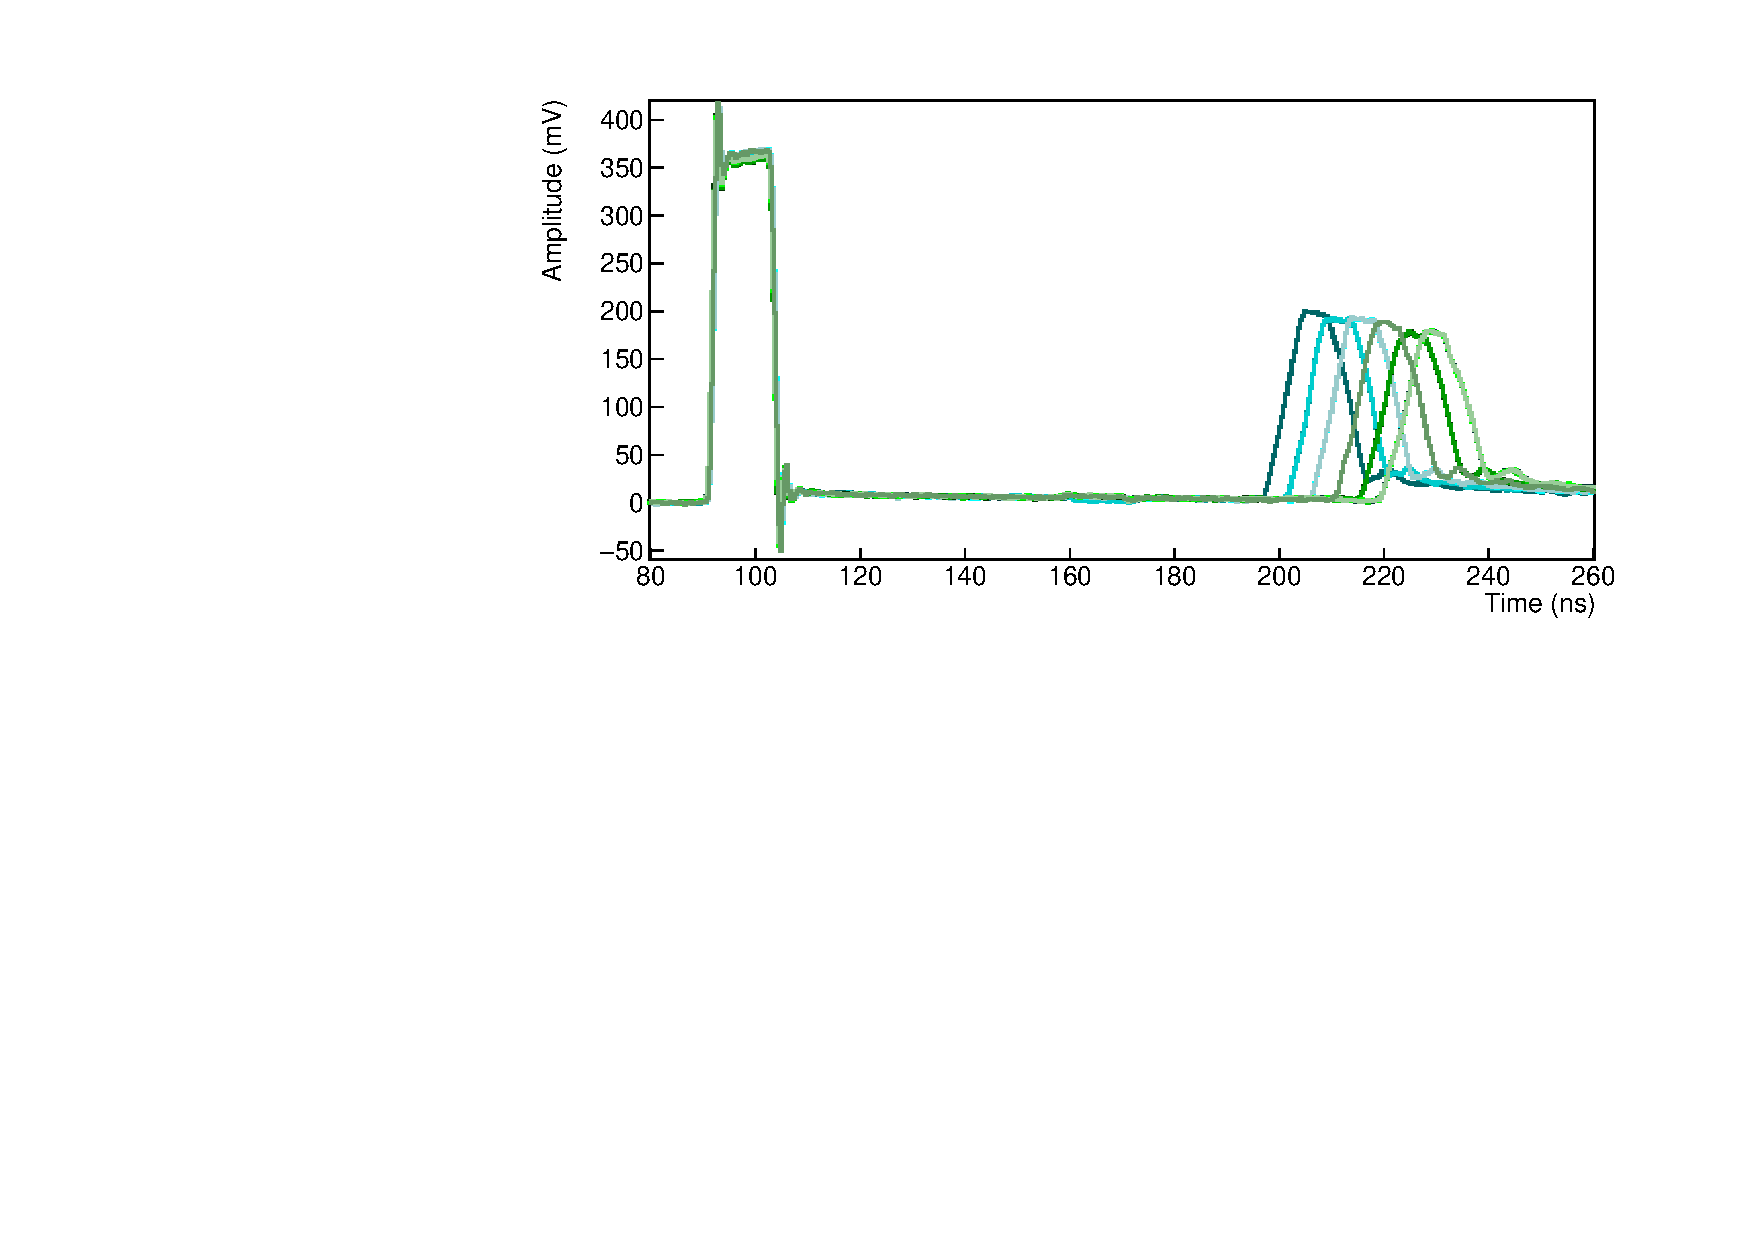
\includegraphics[width=1\textwidth]{commissioning/fig_commissioning/pulses_example.pdf}
  \caption{Primary (left) and secondary (right) pulses for different cable lengths under normal cable operating conditions, for $8$ inches PM.
    Such pulse shapes are used as a reference to detect abnormal pulses and thus identify possible defaults.
    \label{fig:total_waveform}}
\end{figure}

In order to accumulate enough statistics, we send thousands of pulses in each coaxial cable.
The analyses of the shape and arrival times of those secondary pulses for each electronic channel is called \emph{reflectometry}, and allow to check the coaxial cable conditions and to control their lengths.
Mathieu Bongrand (LAL) and me took care of the data acquisition at Modane.

%% Comment les pulses vont être affectés: mettre pulse shape analysis avant.
%% Certains pb déco élec résolus


\subsection{Pulse shape analysis}
\label{subsec:pulse_shape}

By analysing the shape of secondary pulses, one may gather information about the cable state and connection.
This analysis was conducted jointly with Mathieu Bongrand.

In Fig.~\ref{fig:pulse_ex} are displayed three examples of expected secondary pulse shapes, taken as reference in order to compare them with other reflected signals.
These are obtained by averaging all pulses sent in a given electronic channel.
The first one corresponds to a normal recorded pulse for a signal reflected on a $5$ inches PM divider.
The shape is modified compared with the one of $8$ inches, because the impedances at $8$ and $5$ inches dividers are not the same.
The second one is observed when the coaxial cable is misconnected (typically when signal and ground connectors are inverted at PM divider).
The last one stands for a disconnected cable, at the patch panel or photomultiplier, as the signal is being reflected at the end of the coaxial cable.
A reflection at the patch panel level can also be tagged by using pulse timing: the secondary pulse would be detected highly earlier than expected.
Then, a simple check onsite can confirm this observation, and the coaxial cable can be connected again.
\begin{figure}[h!]
  \centering
  \begin{subfigure}[b]{1\textwidth}
    \centering
    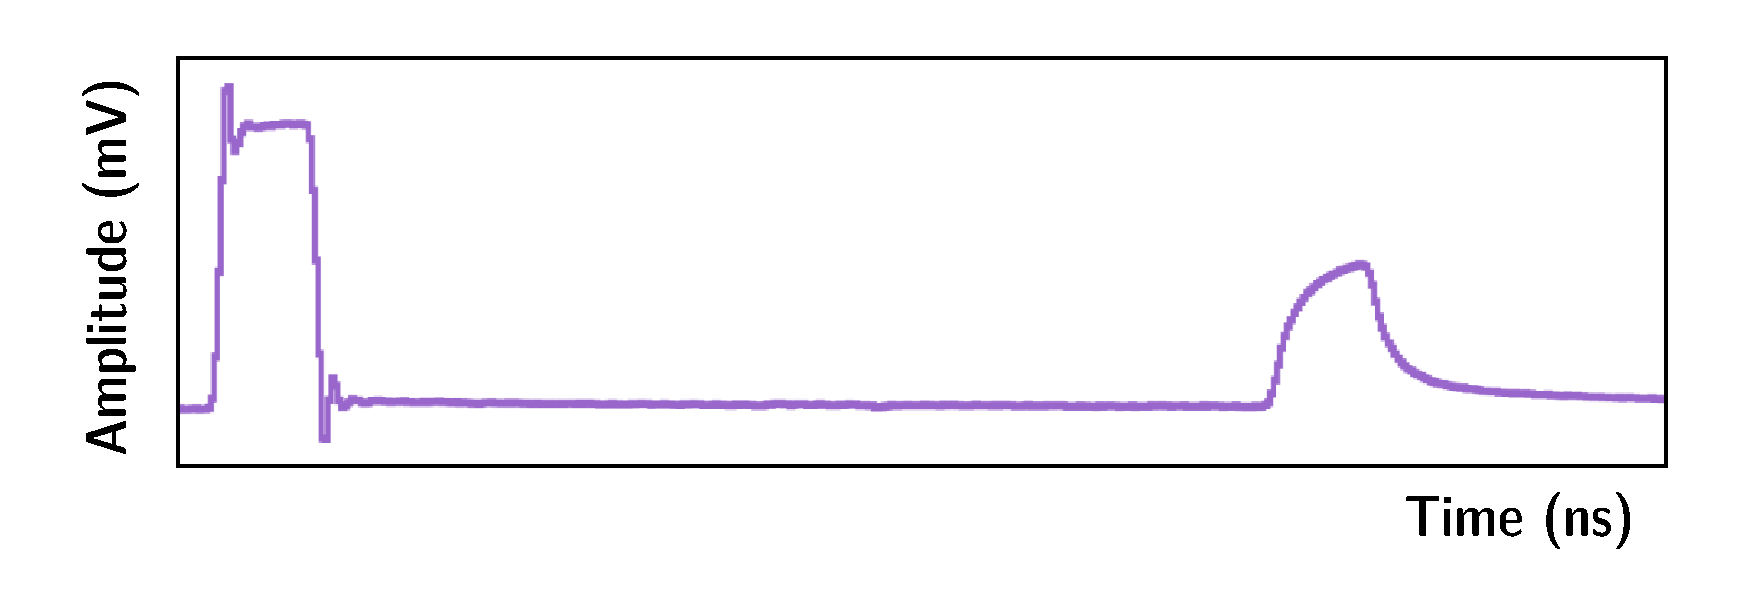
\includegraphics[width=0.7\textwidth]{commissioning/fig_commissioning/normal_pulse_5.pdf}
    \captionsetup{justification=centering}
    \caption{Expected secondary pulse for $5$ inches PM.
      \label{subfig:normal_5}}
  \end{subfigure}
  \begin{subfigure}[b]{1\textwidth}
    \centering
    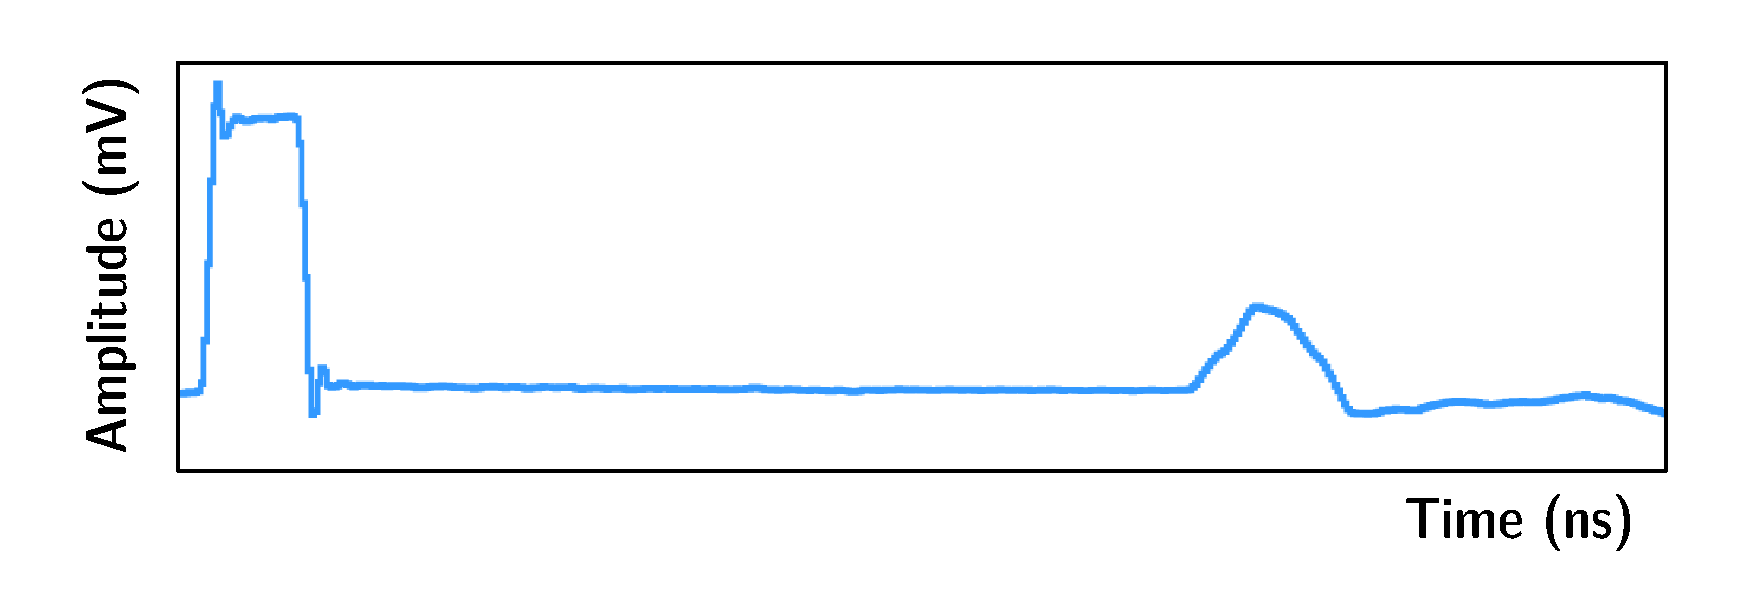
\includegraphics[width=0.7\textwidth]{commissioning/fig_commissioning/anormal_pulse.pdf}
    \captionsetup{justification=centering}
    \caption{Expected secondary pulse for swapped cables at PM.
      \label{subfig:}}
  \end{subfigure}
  \begin{subfigure}[b]{1\textwidth}
    \centering
    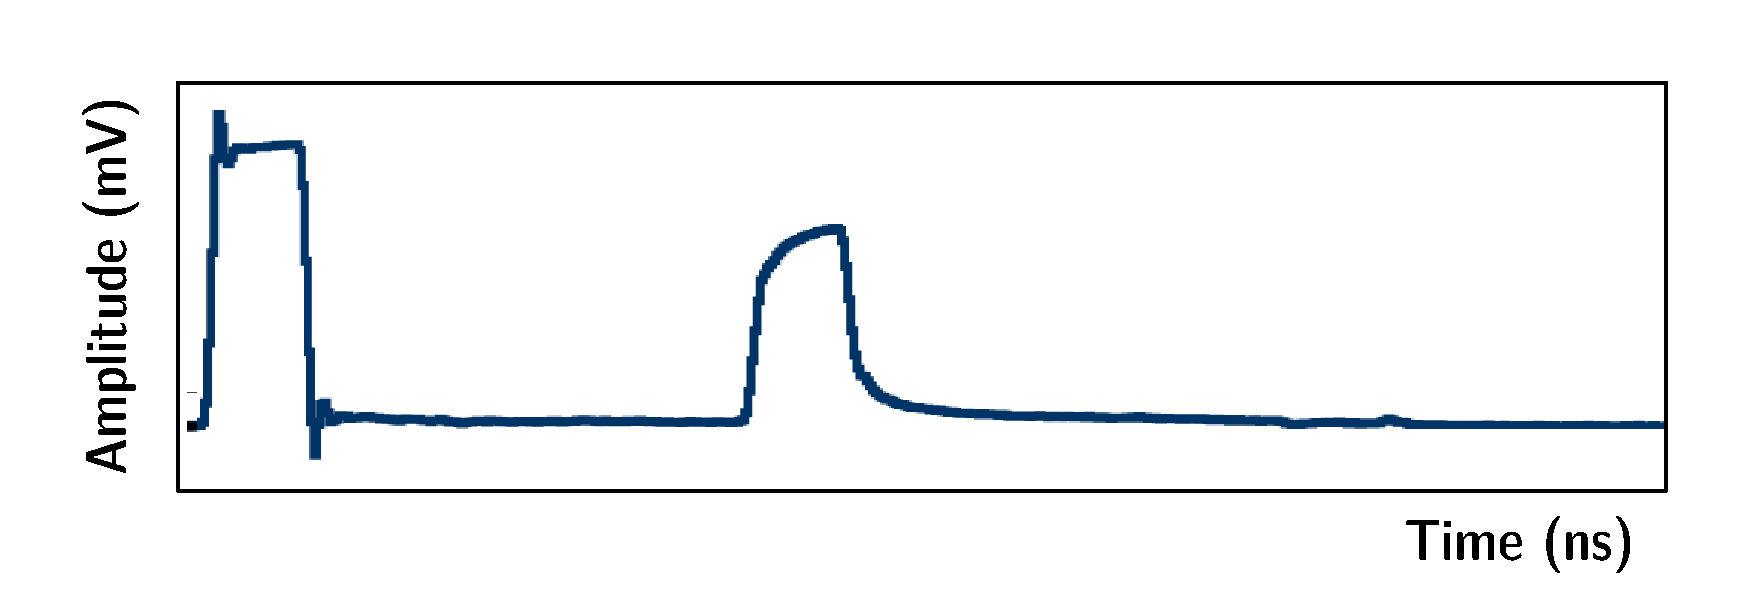
\includegraphics[width=0.7\textwidth]{commissioning/fig_commissioning/anormal_pulse_misco.pdf}
    \captionsetup{justification=centering}
    \caption{Expected secondary pulse for disconnected cable (PP or PM).
      \label{subfig:}}
  \end{subfigure}
  \caption{Expected secondary pulse shapes obtained by averaging the thousands of pulses sent in one cable.
    \label{fig:pulse_ex}}
\end{figure}

In order to identify cabling issues, secondary pulses are averaged for each channel and visually analysed.
If an averaged pulse is identified as abnormal, then the problem affecting the cable can be characterised by comparing the averaged waveform with the references presented.
Thanks to this analysis, some cable de- or misconnections at the patch panel and PM divider have been identified and fixed.

A last issue, which is not pictured in the previous figure, would be if a coaxial cable is damaged in the middle of its length.
In that case, we expect to see pre-pulses between the primary and secondary pulses, stating that a part of the signal is reflected on a cable defect.
The time difference between the initial pulse and the pre-pulse would make it possible to locate the defect.
Such signal has not been observed, leading to the conclusion that no cables have been damaged during transport.

For a future study, it would be interesting to automate this process, as it was done for the analysis presented in Sec.~\ref{subsec:SN_pulse_shape}.
Many manipulations still take place at Modane, some of them close to the calorimeter, which is not yet protected.
It is therefore important to do again these tests before encapsulating the detector.

\subsection{Pulse timing}
\label{subsec:timing}

Coaxial cable lengths have been designed to match the cable routing plan from the electronics to optical modules.
Using the reflectometry tests performed at Modane, we are able to measure precisely each cable length and to compare it with the designed one.

The measured length $l_{j}^{m}$ of a cable $j$ can be defined as
\begin{equation}
  l_{j}^{m}= 0.5\,t_{j}\,v_{p}\, ,
\end{equation}
where $t_{j}$ is the time taken by the signal to make a back and forth trip in the cable, and $v_{p}$ is the signal velocity in coaxial cables.
The time $t_{j}$ corresponds to the averaged timing difference between primary and secondary pulses and is written as
\begin{equation}
  t_{j} = \braket{t_{\text{sec}}-t_{\text{prim}}}_{p} \, \text{,}
  \label{eq:t_j}
\end{equation}
$\braket{}_{p}$ being the average over all pulses sent in one single cable $j$.
The velocity $v_{p}$ can be expressed as a fraction of light speed in vacuum, $c$, as
\begin{equation*}
  v_{p}=\frac{c}{\sqrt{\epsilon_{r}}}\,\text{,}
\end{equation*}
with $\epsilon_{r}$ the relative dielectric constant of the material, indicating that the signal velocity depends on the cable components.
For coaxial cables chosen for SuperNEMO, the manufacturer supplies ${v_{p}=0.69\,c}$.

\subsubsection*{Definition of the pulse timing}

Both analyses of chapters~\ref{ch:sensitivity} and~\ref{ch:timediff} have been performed on simulated data.
The reconstruction software of SuperNEMO does not offer the possibility to reconstruct signal waveforms, and only observables such as the measured energy and time are available.
Nevertheless, as we analyse real data in this chapter, it is an opportunity to describe how the time of an event is defined from the waveform sampling.

The SNFee software, developed by the team in LPC Caen, provide a timing measurement called Constant Fraction Discriminator (CFD), furnishing an amplitude-independent definition of waveform timing.
This algorithm aims at tracking a signal and defining its time at a given fraction $f_{CFD}$ of its maximal amplitude.
The main advantage of this technique is that it provides a good resolution on the measured time.
A graphic representation of the CFD method is given in fig.~\ref{fig:CFD} for $f_{CFD}=40$\%, applied on a secondary pulse.
\begin{figure}[h!]
  \centering
  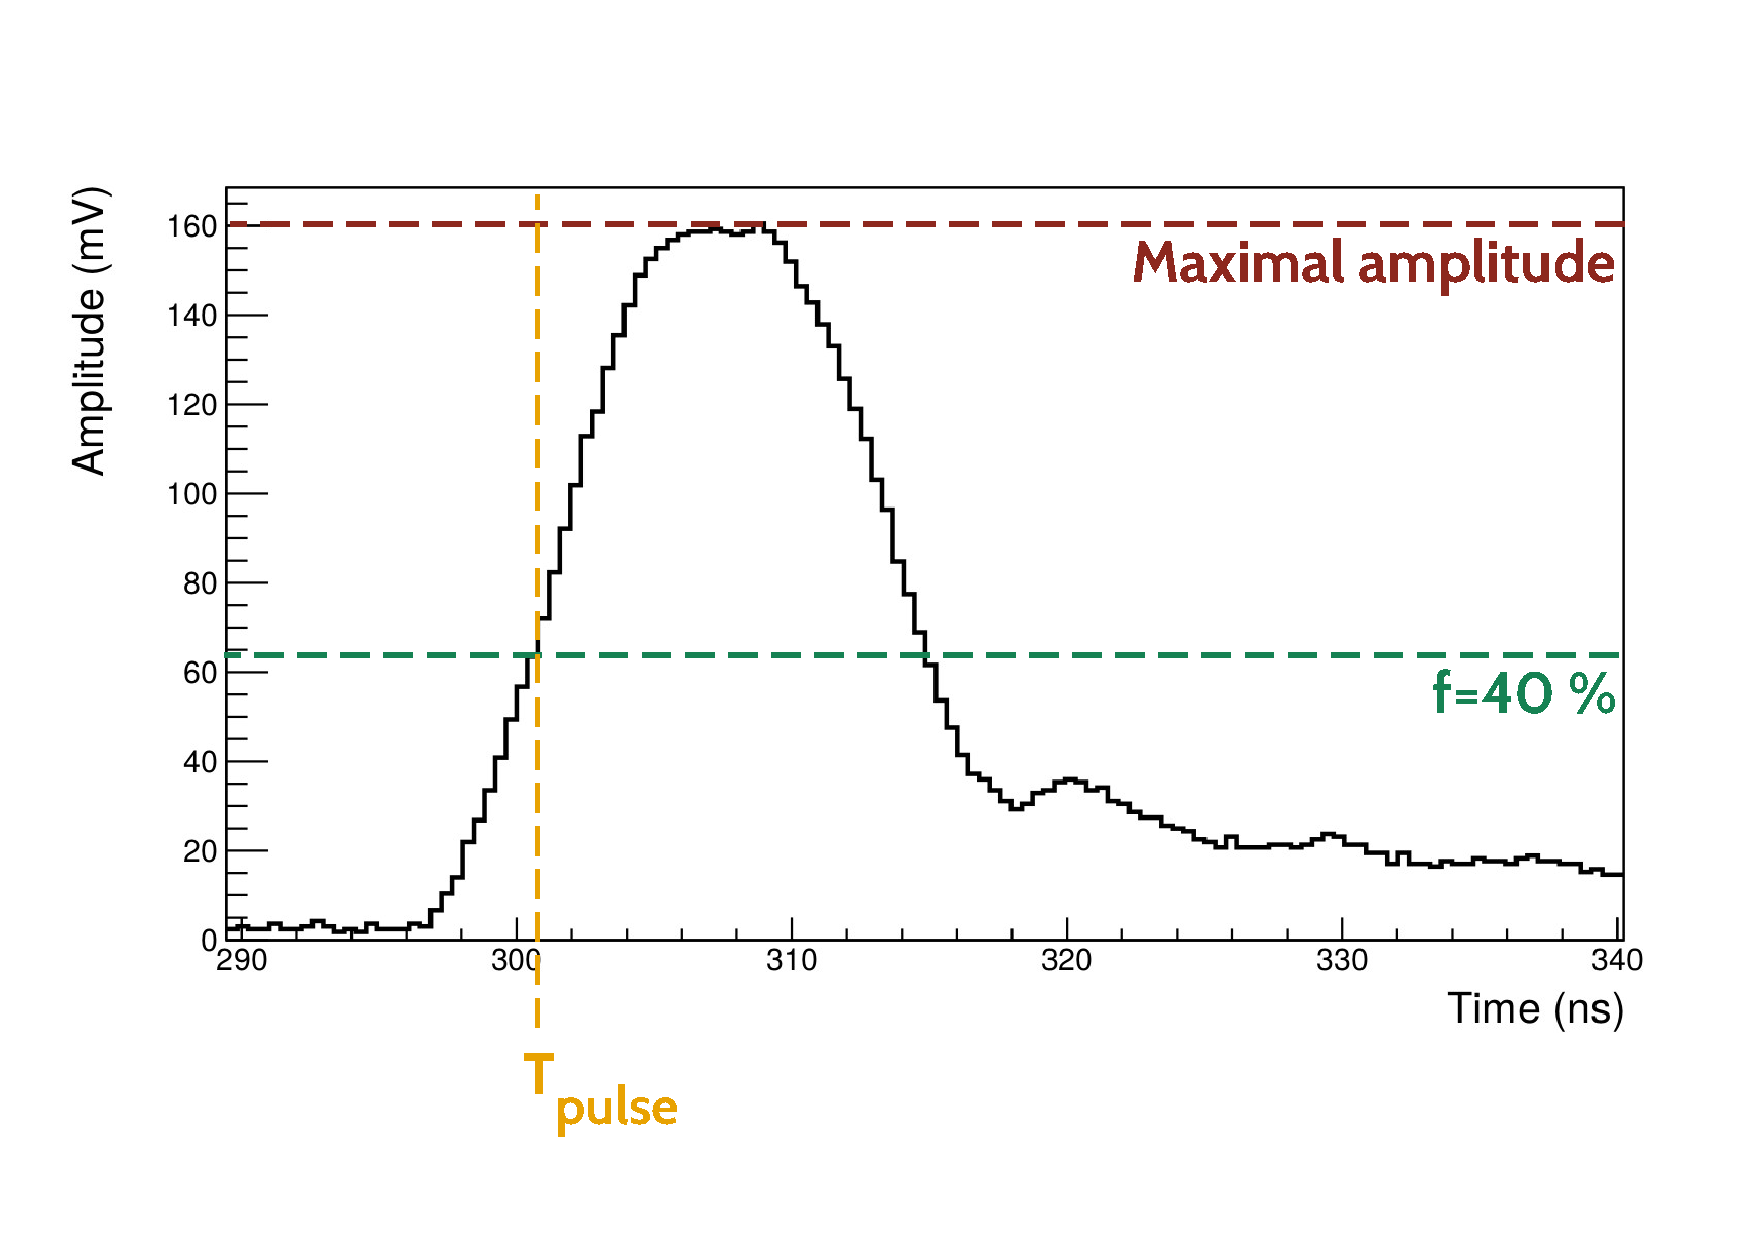
\includegraphics[trim={1.2cm 1.5cm 1.7cm 3.1cm},clip,width=0.7\textwidth]{commissioning/fig_commissioning/CFD_example_zoom.pdf}
  \caption{Graphical representation of the Constant Fraction Discriminator (CFD) method.
    The pulse maximal amplitude (red dotted line) and the fraction $f_{CFD}=40\%$ (green dotted line) are displayed.
    The time $\text{T}_{\text{pulse}}$ (orange dotted line) represents the time defined with this technique.
    \label{fig:CFD}}
\end{figure}

In order to have the best precision on the time measurement, it is important to investigate the possible influence of the $f_{CFD}$ parameter.
An easy operation has been set up at Modane: the coaxial cable connected at a given PM has been split in two parts, connected to two different channels, and electronic pulses were sent through one of the two connected channels.
Therefore, the electronic signal sent in that channel travels through the split cable to the PM and come back to the front-end board.
The signal then slits up to trigger both the two connected channels.
As the signal takes two paths of slightly different lengths, the time difference $\Delta t$ between the two channels can be defined as
\begin{equation}
  \Delta t = t_{ch1}-t_{ch2}\,,
\end{equation}
where $t_{j}$ are defined with Eq.\eqref{eq:t_j} and depends on the $f_{CFD}$ fraction.
In Fig.~\ref{fig:deltat_CFD} is displayed such distributions: three different values of the $f_{CFD}$ parameter are used to compute the $t_{j}$ times, thus giving three different $\Delta t$ distributions.
The means and widths of these distributions depend on $f_{CFD}$.
The distribution width expresses the precision with which time is measured, so this parameter has to be minimised.
In Fig.~\ref{fig:CFD_study} is displayed the distribution width with the value of $f_{CFD}$.
It arises the value giving the best precision on timing measurement is $f_{CFD} = 50\%$ with $\sigma\sim70$~ps, and we adopt this value for the following analysis.
\begin{figure}[h!]
  \centering
  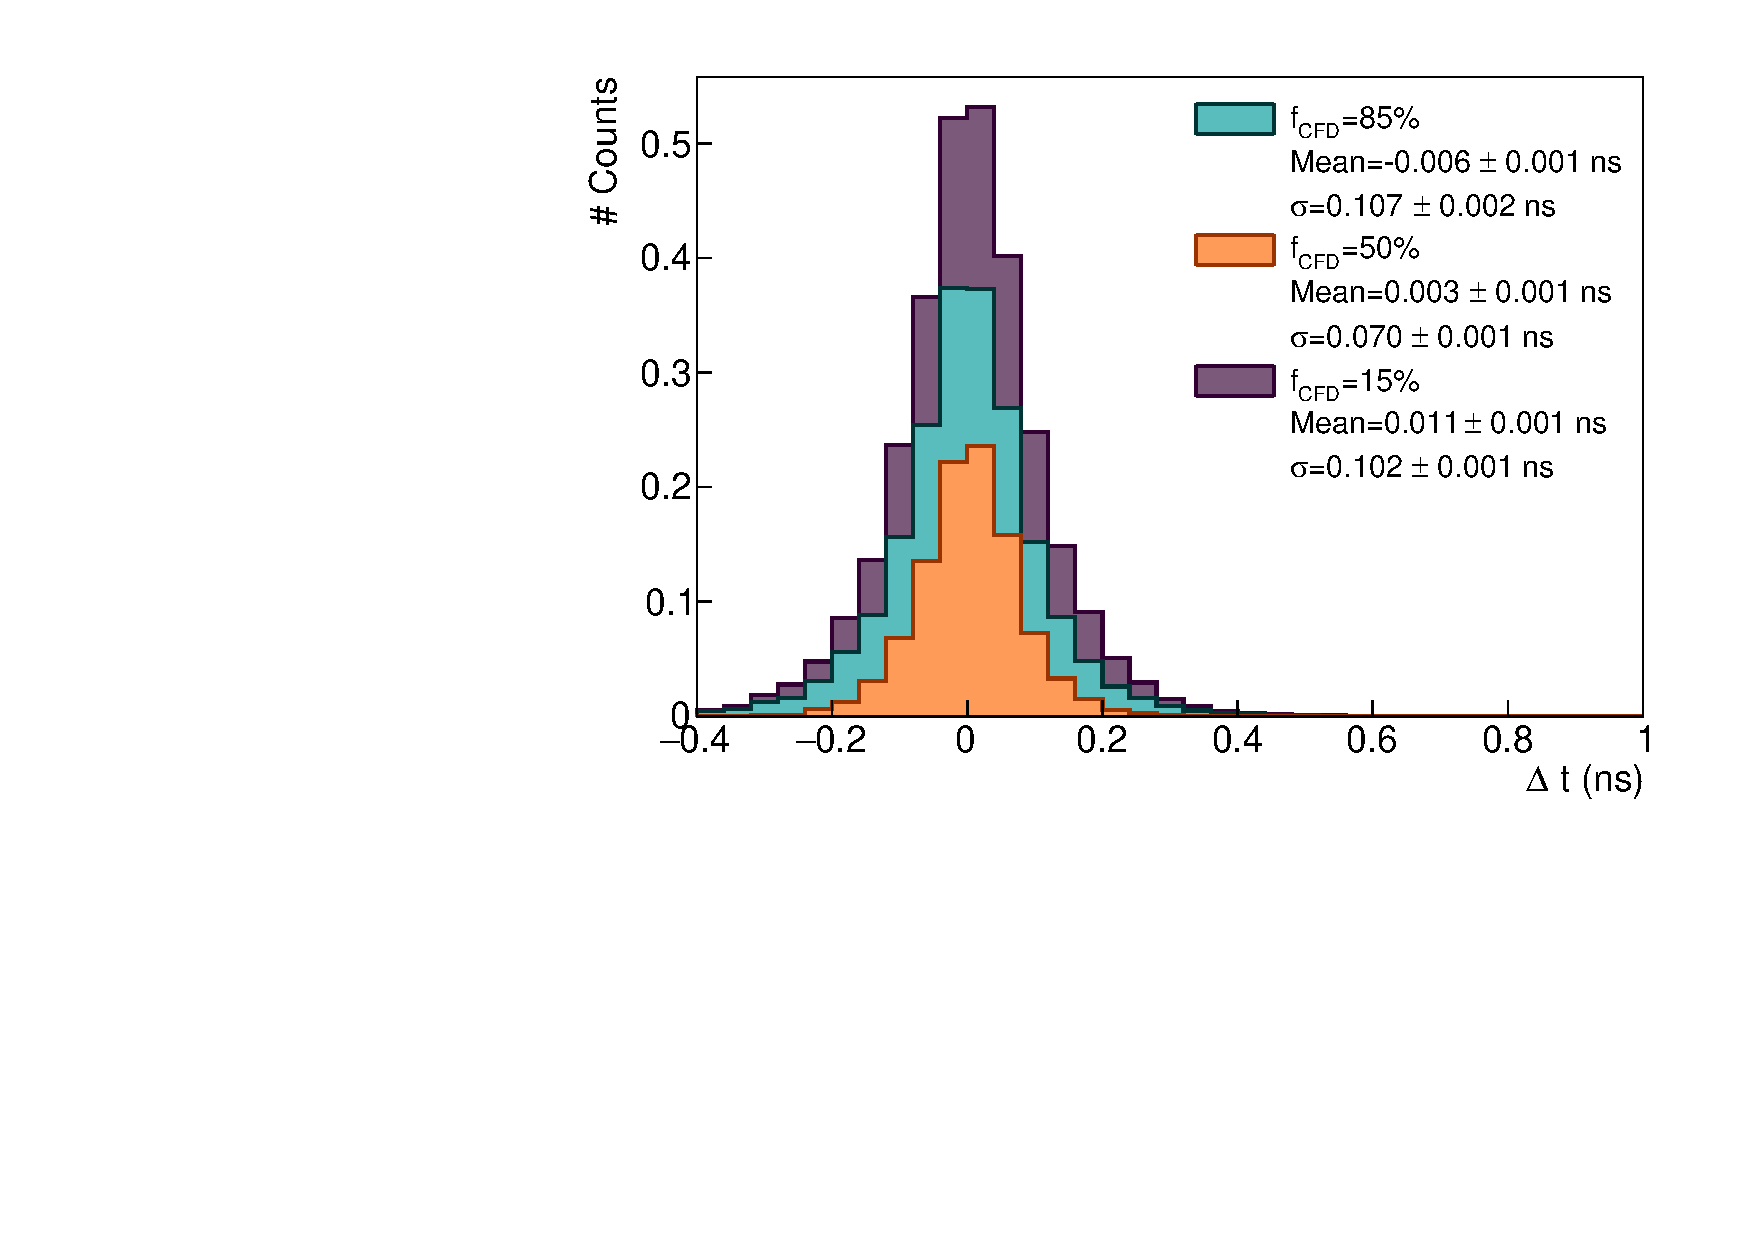
\includegraphics[width=0.7\textwidth]{commissioning/fig_commissioning/deltat.pdf}
  \caption{$\Delta t$ distributions for three different $f_{CFD}$ parameter value.
    \label{fig:deltat_CFD}}
\end{figure}
\begin{figure}[h!]
  \centering
  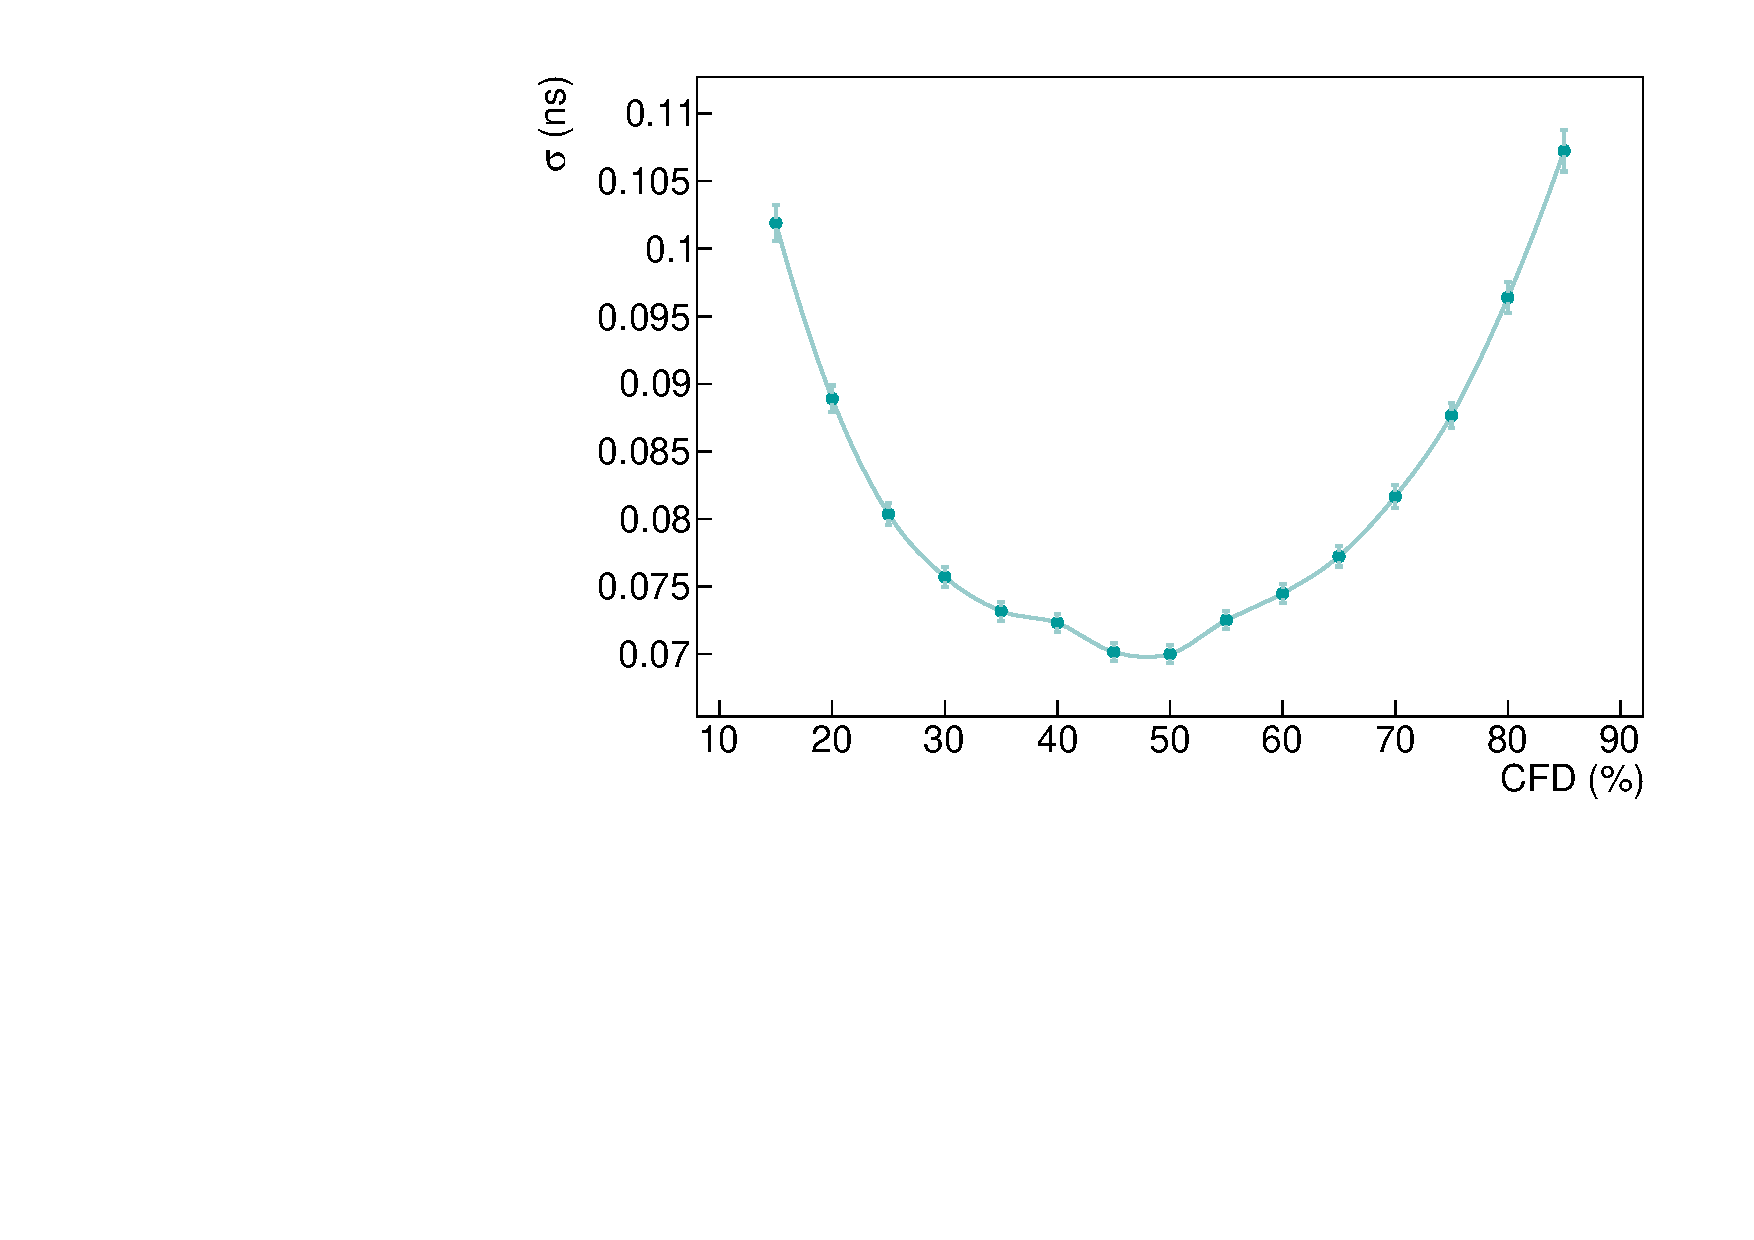
\includegraphics[width=0.7\textwidth]{commissioning/fig_commissioning/CFD_study.pdf}
  \caption{$\Delta t$ distribution width as a function of $f_{CFD}$.
    \label{fig:CFD_study}}
\end{figure}

The signal travels the same path from the PM to the point of cable separation.
The phase shift that occurs between the two paths is caused by the length difference between the two strands of the split cable, as well as the signal path difference within the FEBs calo.
The measurement of the shift for each calorimeter FEB is addressed in Sec.~\ref{sec:timing_FEB}.

\subsubsection*{Signal velocity in coaxial cables}

The value supplied by the manufacturer for signal velocity in coaxial cables is experimentally verified, in order to provide robust and precise results for the reflectometry analysis.

To control this velocity, three coaxial cables of different lengths are measured, with a precision of $1$ cm.
A thousand of electronic pulses are sent in each of the three cables and secondary pulses are recorded.
The time $t_{j}$ is then measured, using the CFD method.
In Fig.~\ref{fig:celerity} is displayed the lengths $l_{j}$ as a function of the times $t_{j}$.
This procedure allows to have three independent measurements for the signal velocity by fitting these points.
The value of $v_{p}/c = 0.697\pm 0.0011$ is found, showing a compatibility up to $7\sigma$ with the data sheet.
Certain conditions during data acquisition may explain this difference, such as the frequency of the signal.
This velocity is kept for the current analysis.
\begin{figure}[h!]
  \centering
  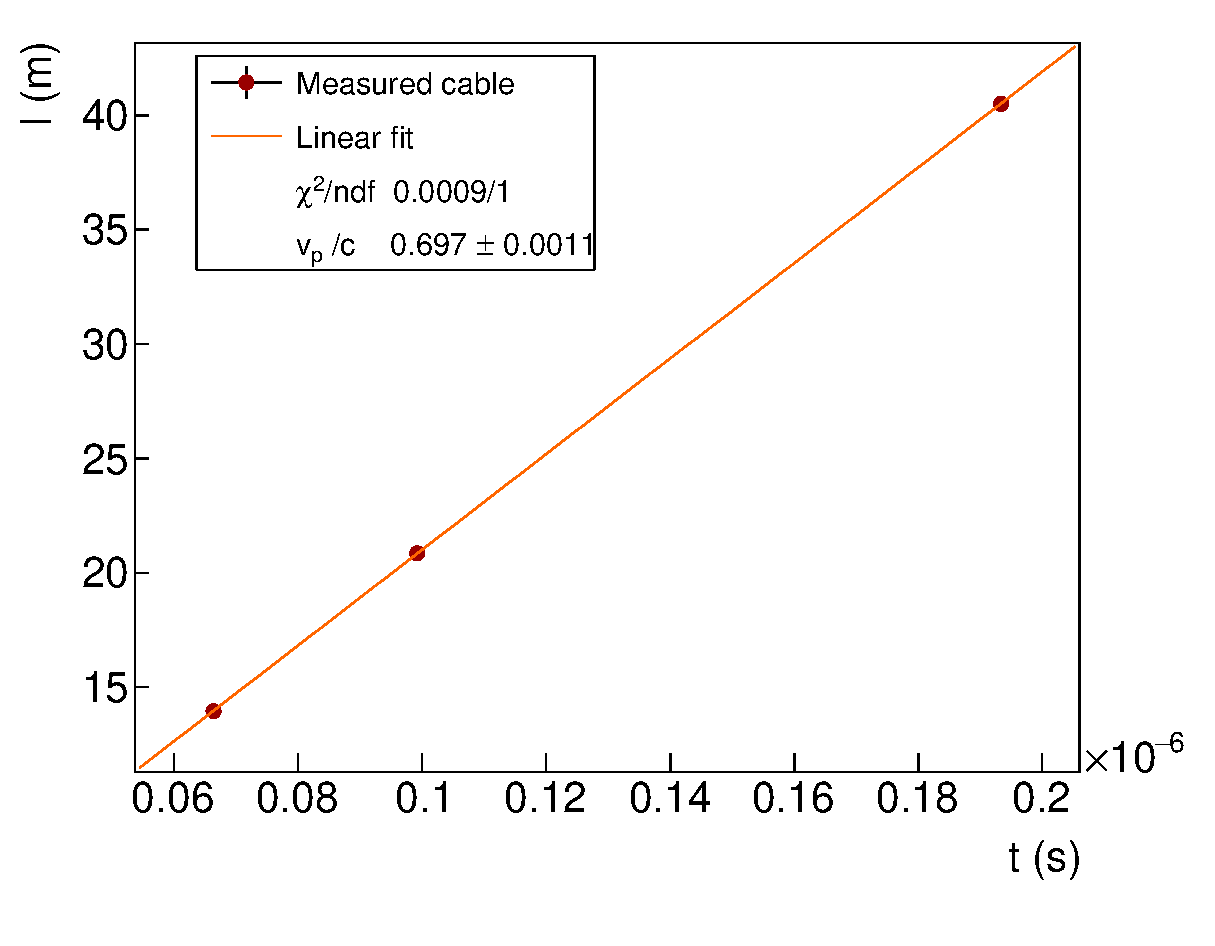
\includegraphics[width=0.7\textwidth]{commissioning/fig_commissioning/celerity.eps}
  \caption{Three different lengths $l_{j}$ of cables are measured.
    Pulses are sent inside all cables.
    The lengths $l_{j}$ are plotted as a function of the time differences $t_{j}$ between primary and secondary pulses.
    The value of $v_{p}/c$ fitted from the data points is displayed.
    This value of $0.697\pm 0.0011$ shows the compatibility with the one supplied by the constructor, of $0.69$ c.
    \label{fig:celerity}}
\end{figure}

\subsubsection*{Cable lengths}

One of the principal goal of this study is to measure the cable lengths $l^{m}_{j}$ using reflectometry data, in order to check if they were cut at designed lengths $l^{d}_{j}$.
Results are presented for main wall cables.

Coaxial cables are tested by sending pulses in front-end boards electronic channels, and by measuring the secondary pulse times.
The length difference $\Delta L_{j}$ between measurements and expectations is defined as
\begin{equation}
  \Delta L_{j} = l^{m}_{j}-l^{d}_{j}\,.
\end{equation}
Knowing the signal velocity inside cables, each cable length is determined precisely.
In Fig.~\ref{fig:LengthDiff} is displayed the distribution $\Delta L$ of lengths measured by reflectometry.
In hypothetical perfect conditions, all tested cables should have the designed length, in other words, $l^{d}_{j} = l^{m}_{j} \;\forall j$.
In that case, the $\Delta L$ distribution would be a Dirac peak at zero.
However, in real conditions, the measured lengths are different from the designed one, leading an enlargement of the distribution.
This width gives access to the cutting device precision, measured at $\sigma=5.0\pm0.3$~cm, which is an acceptable value for the cable length accuracy required.
A few cables have been cut too short by mistake, the worse of them being $80$ centimetres shorter than expected.
A verification has been made on site to check a possible disconnection at the patch panel, but it turned out that this cable had indeed been cut too short.
Fortunately, this cable  was successfully connected to PM despite this deficit.
On the contrary, few cables have a large extra length.
This probably is due to human punctual mistakes, but without any strong consequences for the calorimeter operation.
\begin{figure}[h!]
  \centering
  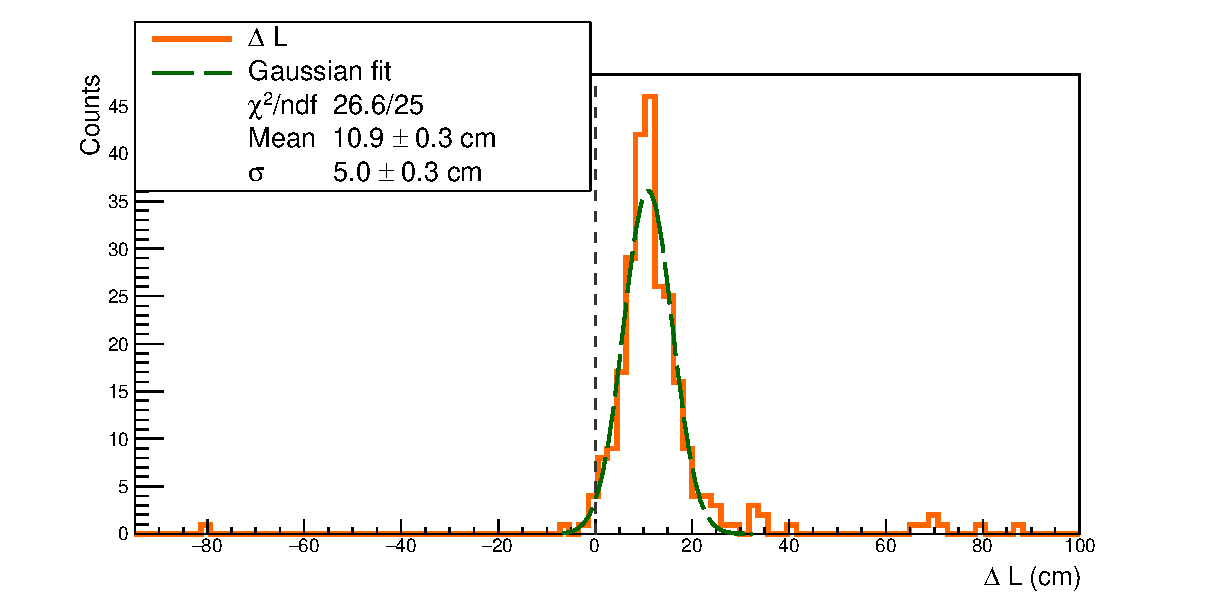
\includegraphics[width=15cm]{commissioning/fig_commissioning/length_diff.eps}
  \caption{The $\Delta L$ distribution for coaxial cables of the two main calorimeter walls (orange).
    The ideal case for which $l^{m}_{j} = l^{d}_{j} \;\forall j$ is displayed (grey dashed line).
    Some data points considered as outliers are beyond $3\sigma$.
    \label{fig:LengthDiff}}
\end{figure}

Surprisingly, the distribution is also shifted towards positive values, with the mean at $+10.9\pm 0.3$ cm, meaning that cables are longer than expected, in average.
This may reveal a bias coming from the cable cutting device.
Indeed, during the cutting process, the device had a tendency to slip, probably leading to extra lengths of cable.
If that is the case, we assume the device has a determined probability to slip, for one meter of cable.
Therefore, the probability for the device to provide extra length should increase with the cable length.
To verify this assumption, Fig.~\ref{fig:CutBias} displays the length difference $\Delta L$ as a function of the initial design length $l^{d}$.
A linear fit, parameterised as $y = \alpha x + \beta$, reveals that the cutting device presents two different biases.
The value of $\beta$ shows that it systematically takes away $3.4$ cm of each cable.
As it was planned in the design to add a few tens of centimetres per cable, for safety reasons, this bias is absorbed and is not a cause of concern.
Besides, the slope $\alpha = 0.010\pm 0.002$ of the linear fit reveals that one extra centimetre is added for every meter of cable, being compatible with the hypothesis on the cutting device sliding.
Hopefully this bias is not problematic as it makes most of the actual cable lengths longer than the design, while shorter lengths could have led to systematic connection issues to PMs.
In conclusion, no important mistakes have been made when cutting cables, and we had no issue for connecting the only problematic cable.
\begin{figure}[h!]
  \centering
  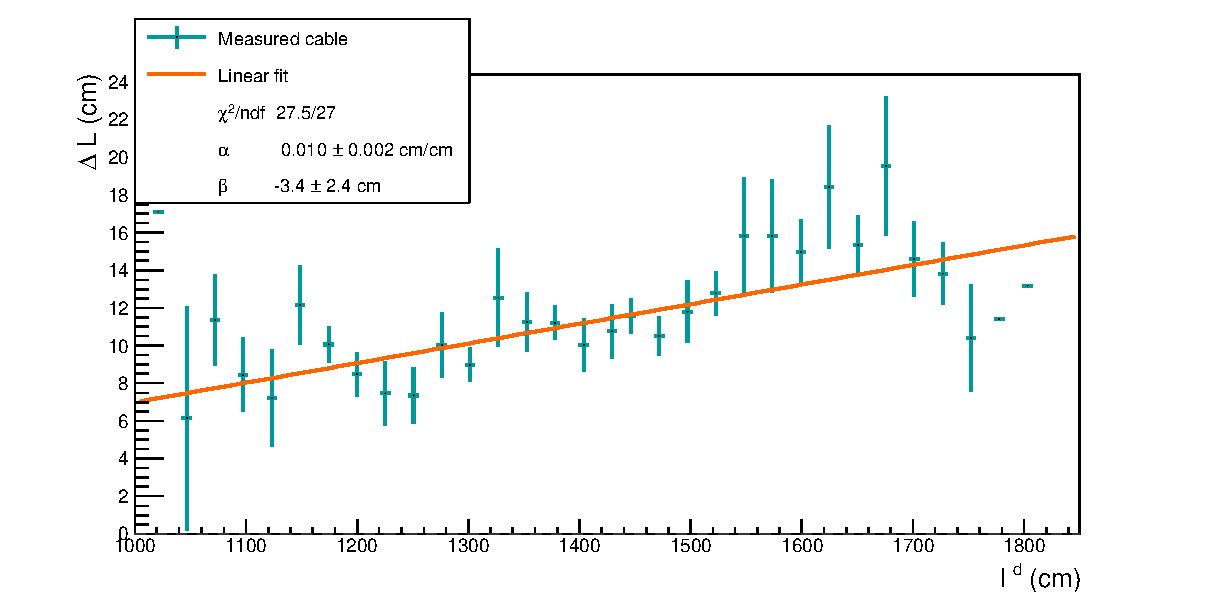
\includegraphics[width=15cm]{commissioning/fig_commissioning/cut_biais.eps}
  \caption{$\Delta L$ values as a function of $l^{d}$ (cyan), where $l^{d}$ are averaged in each bin.
    Data points are fitted by $\alpha x + \beta$, with $\alpha > 0$ and $\beta < 0$, revealing the two biases of the cutting device.
    \label{fig:CutBias}}
\end{figure}

The analysis of reflectometry data allowed to find and repair damaged coaxial cables, as well as to measure their length, thus taking part in the commissioning effort that has been provided by the whole collaboration.
Measuring the real cable lengths give also access to the time taken by the signal to go from a PM to the electronics, which is an important characteristic of the demonstrator, that has to be characterised.

\subsubsection*{Signal time delay}

Once the signal velocity is measured, the time needed for the signal to travel from one given PM divider to the electronic boards can be deduced.
This time travel induces a signal delay, specific to each electronic channel.
Therefore, one of the greatest implication of this study was to provide for the collaboration a database containing time delays for each electronic channel of the two main walls.
This document is available on the Lyon computing platform.


\subsection{Signal attenuation}
\label{subsec:attenuation}
The attenuation of an electric signal is a problem common to all electronic fields, and comes from the charge absorption of an electromagnetic wave travelling in a medium.
%% Then, another test for controlling the cable condition is to check if this attenuation matches
%% the expectations (i.e. the attenuation per metre of cable given by constructor).
%% The signal attenuation car be define in two different ways:
%% \begin{itemize*}
%% \item using the signal amplitude ratio
%% \end{itemize*}
For a coaxial cable, this attenuation mainly depends on the signal frequency $f$ in MHz and on the cable characteristics.
For the coaxial cables, the theoretical linear attenuation $\alpha_{\text{att}}^{\text{th}}$ corresponds to the attenuation by metre of cable in dB/m.
It is supplied by the constructor as
\begin{equation}
  \alpha_{\text{att}}^{\text{th}} = f\sqrt{\epsilon}(\frac{a}{\sqrt{f}}+b)\,,
\end{equation}
where the factor $a$ depends on the diameter of the dielectric material on one side, and of the diameter of the conductor material on the other side, and where $b$ is function of the dielectric loss factor, characterising the material's dissipation of electromagnetic energy.
For the used coaxial cables, and with a frequency $f$ of few GHz for the signal pulses sent in cables, we calculate this attenuation as $\alpha_{\text{att}}^{\text{th}} = 1.22$ dB/m.
In a more general manner, the attenuation of a signal in dB is defined with the decimal logarithm of a power ratio.
We use this definition to determine the attenuation in the framework of the reflectometry analysis, defining the attenuation $\mathcal{A}$, for a given length of cable $l$, as
\begin{equation}
  \mathcal{A}=10\log_{10}\frac{V_{\text{prim}}}{V_{\text{sec}}} \,\text{,}
\end{equation}
where $V_{i}$ is a quantity representing the intensity of the signal.
It corresponds either to the maximal amplitude of the pulse $A$ or to the pulse charge $Q$, defined as the amount of signal received by the acquisition, integrated over the acquisition time window.
As the provided data sheet does not specify the attenuation of which quantity (amplitude or charge) represents $\alpha_{\text{att}}^{\text{th}}$, we decide to investigate both in the following.
Then, we define the linear attenuation $\alpha_{\text{att}}^{\text{R}}$, measured by reflectometry in dB/m, with
\begin{equation}
  \mathcal{A} = f_{r}+\alpha_{\text{att}}^{\text{R}}\,l\,,
\end{equation}
with $f_{r} = -10\log_{10}R$, where $R$ is the reflection factor characterising the pulse reflection on the PM divider.
In fact, as the circuit is opened, the pulse is reflected at the PM divider, but only partially.
A part of the signal is not reflected but lost through the divider.
This reflection is characterised by $R$, which is function of the impedance $Z_{c}$ of the cable, and of the impedance $Z_{d}$ at the divider level, where the pulse is reflected.
It is written as
\begin{equation}
  R = \frac{Z_{d}-Z_{c}}{Z_{d}+Z_{c}}\,,
\end{equation}
where we have the limit
\begin{equation}
  \lim_{Z_{d} \to \infty} f_{r} = 0 \text{ and } R=1\,,
\end{equation}
expressing a total reflection occurring when the impedance at the PM divider is infinite.
The main goal here is to determine the value of $\alpha_{\text{att}}^{\text{R}}$, using the reflectometry data, and to compare it with $\alpha_{\text{att}}^{\text{th}}$.
Moreover, the impedance $Z_{d}$ value at PM divider can be estimated from the determination of $f_{r}$.
In Fig.~\ref{fig:attenuation} is shown the linear dependence between the attenuation $\mathcal{A}$ and the cable length $l$, for amplitude and charge.
The amplitude $A$ is given in mV and the charge $Q$ in mV.ns.
The values of $\alpha_{\text{att}}^{\text{R}}$ and $f_{r}$, for both amplitude and charge cases, are displayed in the legend.
Firstly, the two linear fits reveal that, whether calculated with the amplitude, or with the charge, the linear attenuation $\alpha_{\text{att}}^{\text{R}}$ is smaller than the calculated one $\alpha_{\text{att}}^{\text{th}}$ (for the amplitude case, $\alpha_{\text{att}}^{\text{th}}\simeq 5\times \alpha_{\text{att}}^{\text{R, amp}}$, and for the charge case $\alpha_{\text{att}}^{\text{th}}\simeq 7\times \alpha_{\text{att}}^{\text{R, ch}}$).
That means the signal is less affected, when transmitted by the cable, than expected.
Secondly, the attenuation in charge is less important that the attenuation in amplitude.
This can be easily explained: as it is integrated over time, the charge is a quantity less affected by amplitude variations that the amplitude itself.
For the same reason, the charge data set points are less spread than the amplitude ones, confirming we are less sensitive to cable length variations when using the charge quantity.
\begin{figure}[h!]
  \centering
  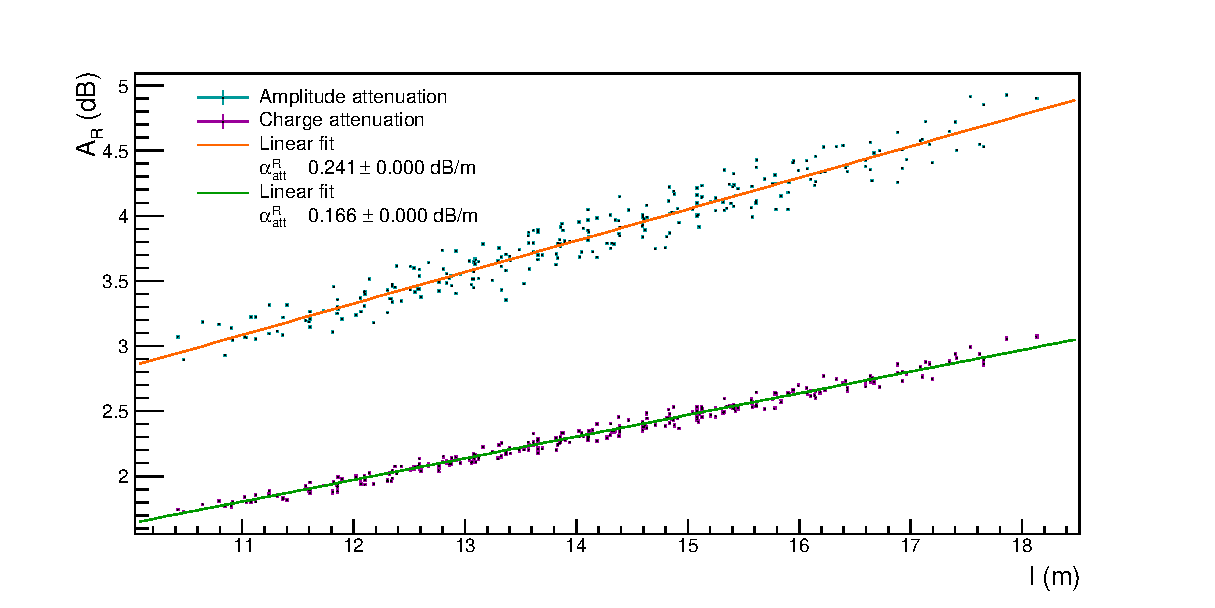
\includegraphics[width=15cm]{commissioning/fig_commissioning/attenuation_length.eps}
  \caption{The amplitude $\mathcal{A}$ is displayed as a function of the measured cable length $l$.
    The data set calculated with the amplitude (charge) is given in cyan (magenta) and fitted by a linear function in orange (green).
    The values of the slope, which represent the linear attenuation of the coaxial cables in dB/m, are respectively $\alpha_{\text{att}}^{\text{R, amp}} = 0.241\pm 0.000$dB/m and $\alpha_{\text{att}}^{\text{R, ch}} = 0.166\pm0.000$dB/m.
    The two $y$-intercept values, which represent the reflection of the pulse on the PM divider, are $f_{r}^{amp} = 0.402\pm 0.032$ dB and $f_{r}^{ch} = -0.020\pm 0.013$ dB.
    \label{fig:attenuation}}
\end{figure}

The study of signal attenuation allows us to conclude that coaxial cables do not significantly degrade the signal transmission, especially if we look at the waveform charge.
However, looking at the shape of the secondary pulses compared to the primary ones, it is clear that the pulse shape, and especially its rising edge, is affected by the path in the cable.
It would then be interesting to conduct a study investigating the influence of these cables on the rising edge time, and thus on the accuracy of time measurement of calorimeter data due to the coaxial cables.

\subsection{Summary}

Analysis of reflectometry data allowed to control the coaxial cables status after the calorimeter cabling operations.
All possible misconnections and damaged connectors have been fixed.
The time measurement, using the CFD method, was optimised in order to have a better timing precision.
All cable lengths were checked and revealed the cutting device is biased, producing cables longer than designed.
The corresponding time delay induced by the signal time travel are stored in a database made available for the collaboration.
This study was the occasion to understand some properties of the cables, as velocity and attenuation of a signal travelling in coaxial cables.

Apart from the coaxial cables, the calorimeter FEBs themselves can have an impact on the signal timing delay, which is addressed in the next section.

\section{Synchronisation of calorimeter FEBs}
\label{sec:timing_FEB}

One of the parameters that can also delay and de-synchronise the signal collected from optical modules is the path difference of the electronic signal inside the calorimeter FEBs, which is pictured in Fig.~\ref{fig:FEB_scheme}.
Indeed, the CB manages the distribution of the clock in all calorimeter FEBs.
The further away the CB is from an FEB on the crate, the longer it will take for this information to be transmitted.
The scheme given is highly simplified and in practice even each electronic channels of a given board has an individual delay.
This de-synchronisation has to be characterised in order to calibrate each electronic channel of each FEB, which is primordial for analysis of coincidence events with the calorimeter.
\begin{figure}[h!]
  \centering
  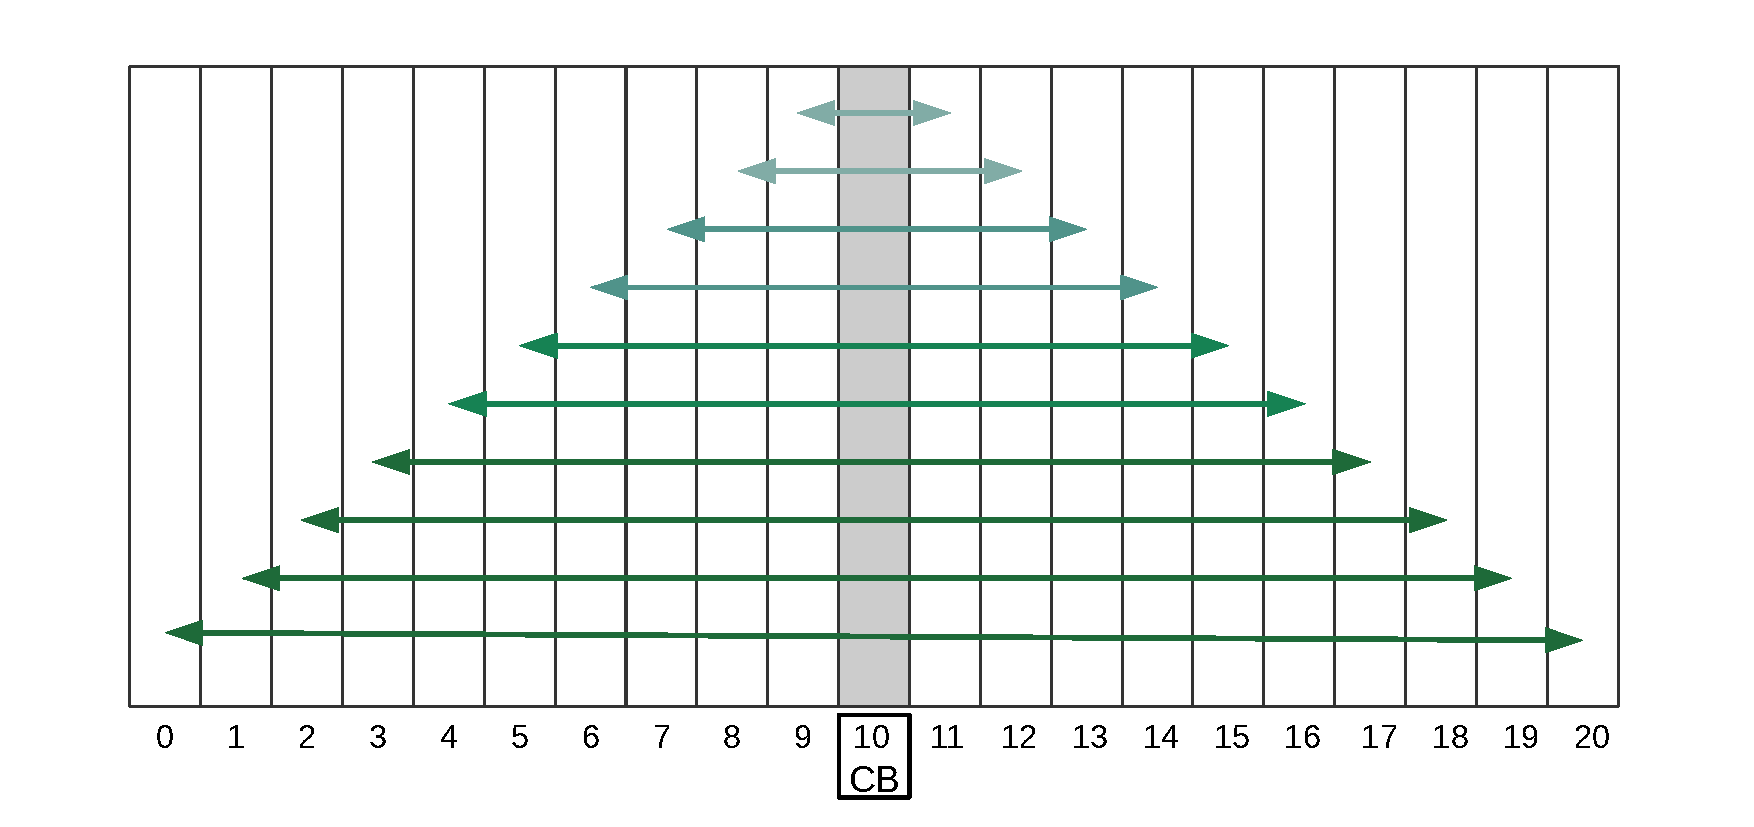
\includegraphics[width=0.9\textwidth]{commissioning/fig_commissioning/clock_distribution_back_plain.pdf}
  \caption{Sketch of the electronic paths from the central CB to each FEB.
    \label{fig:FEB_scheme}}
\end{figure}

The set up used to measure this de-synchronisation was provided by the electronics team at LAL.
A wave-catcher is set up to produce an electronic impulse (of same shape as the one used for reflectometry) and split it in two channels.
By connecting this device on pairs of FEB channels, one can measure the time offset existing between them.
The general principle consists then in choosing a channel taken as a reference by connecting one cable of the device to it.
Then data acquisitions are taken by connecting successively the other cable to all other channels from the same crate, allowing to measure the offset existing between them and the reference channel.
Three examples of $\Delta t$ distributions are given in Fig.~\ref{fig:FEB_offset}, for three different channels belonging to the same FEB, in coincidence with the reference channel.
The distributions $\sigma$ stand around $\sim20-30$~ps and represent the resolution on time measurements brought by the calorimeter FEBs.
The distributions mean represents the time offset of each of the three channels with the channel taken as a reference.
\begin{figure}[h!]
  \centering
  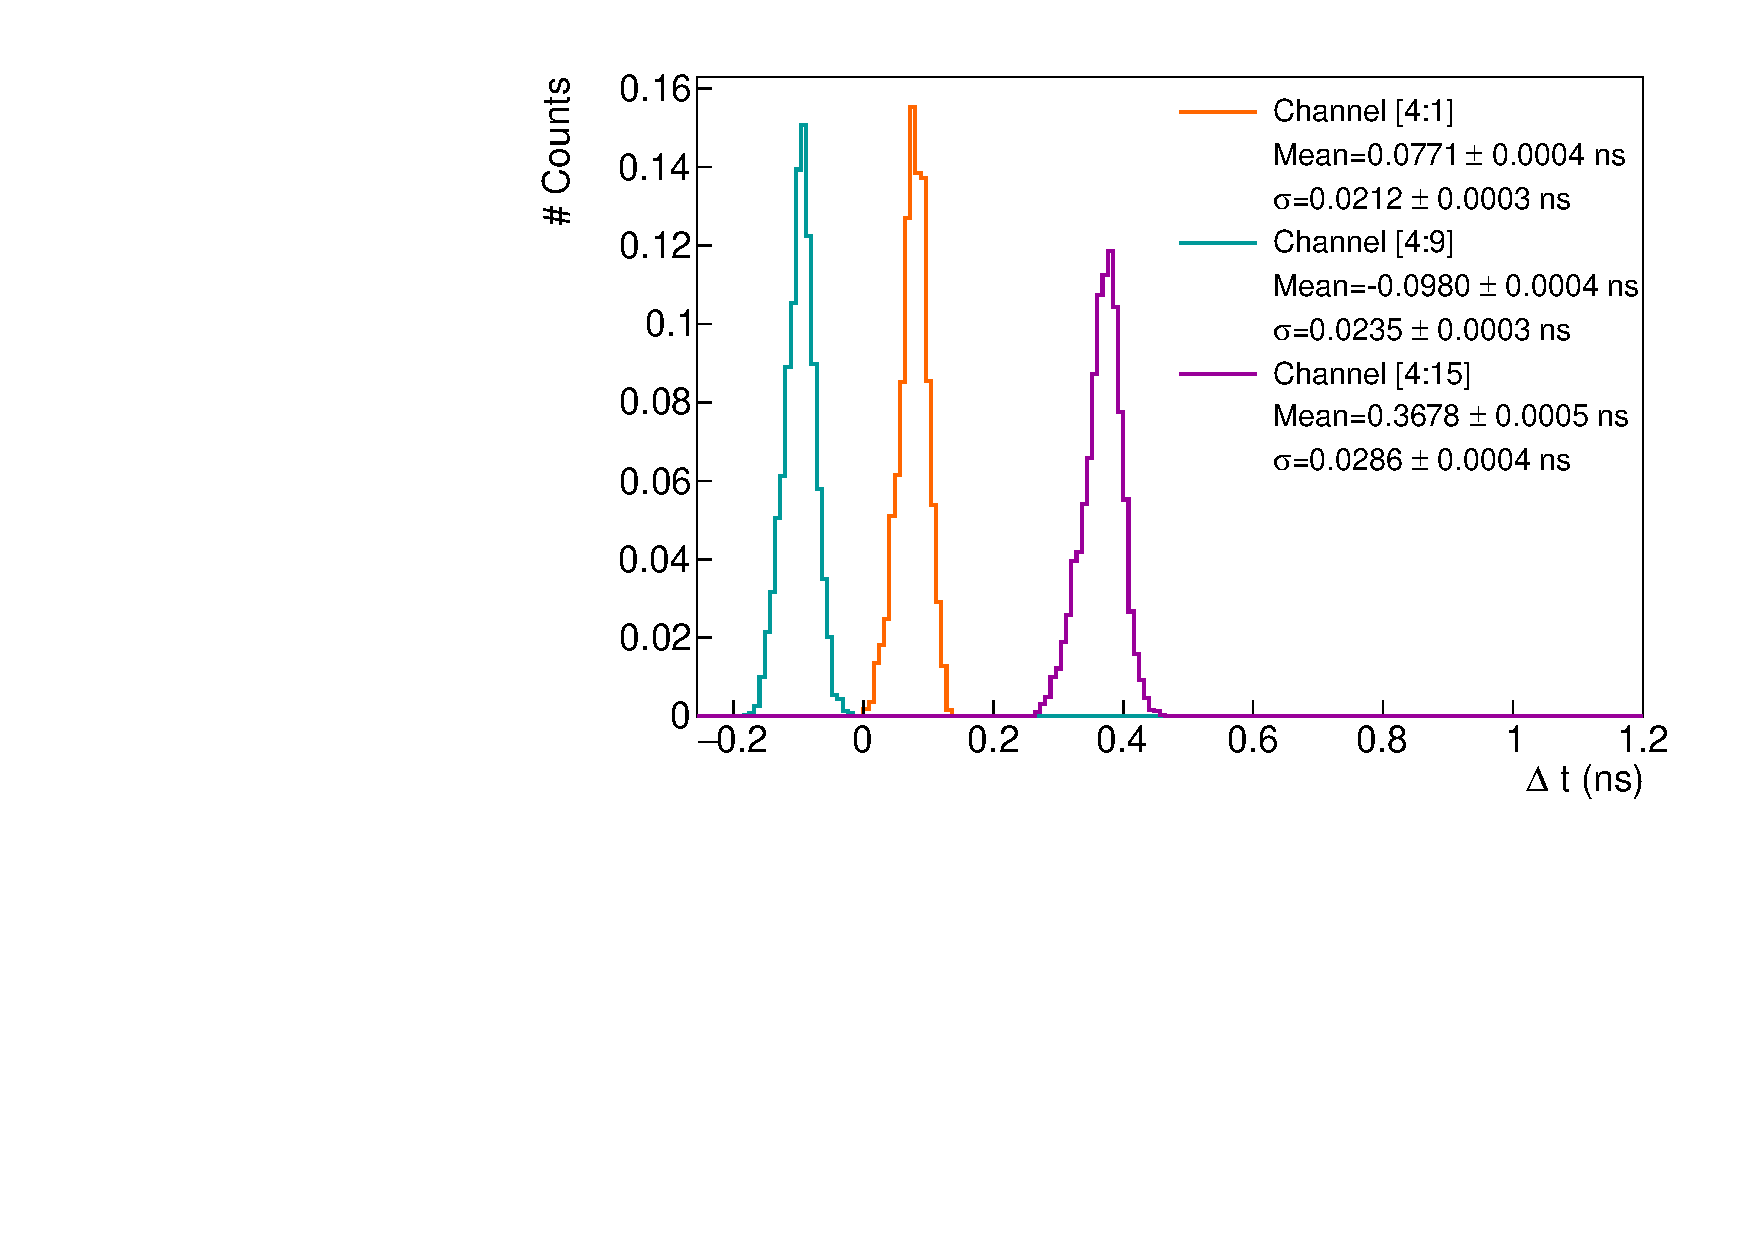
\includegraphics[width=0.7\textwidth]{commissioning/fig_commissioning/time_offset.pdf}
  \caption{$\Delta t$ distributions between the reference channel and three channels on the same FEB.
    \label{fig:FEB_offset}}
\end{figure}

The goal of this analysis is to characterise the time offset of each channel of each FEB.
In Fig.~\ref{fig:mean_distance} is given the mean of the $\Delta t$ distributions as a function of the distance between the corresponding FEB and the central CB.
The more distant an FEB is from CB, the greater its time offset will be in relation to the reference taken, confirming the description given in Fig.~\ref{fig:FEB_scheme}.
\begin{figure}[h!]
  \centering
  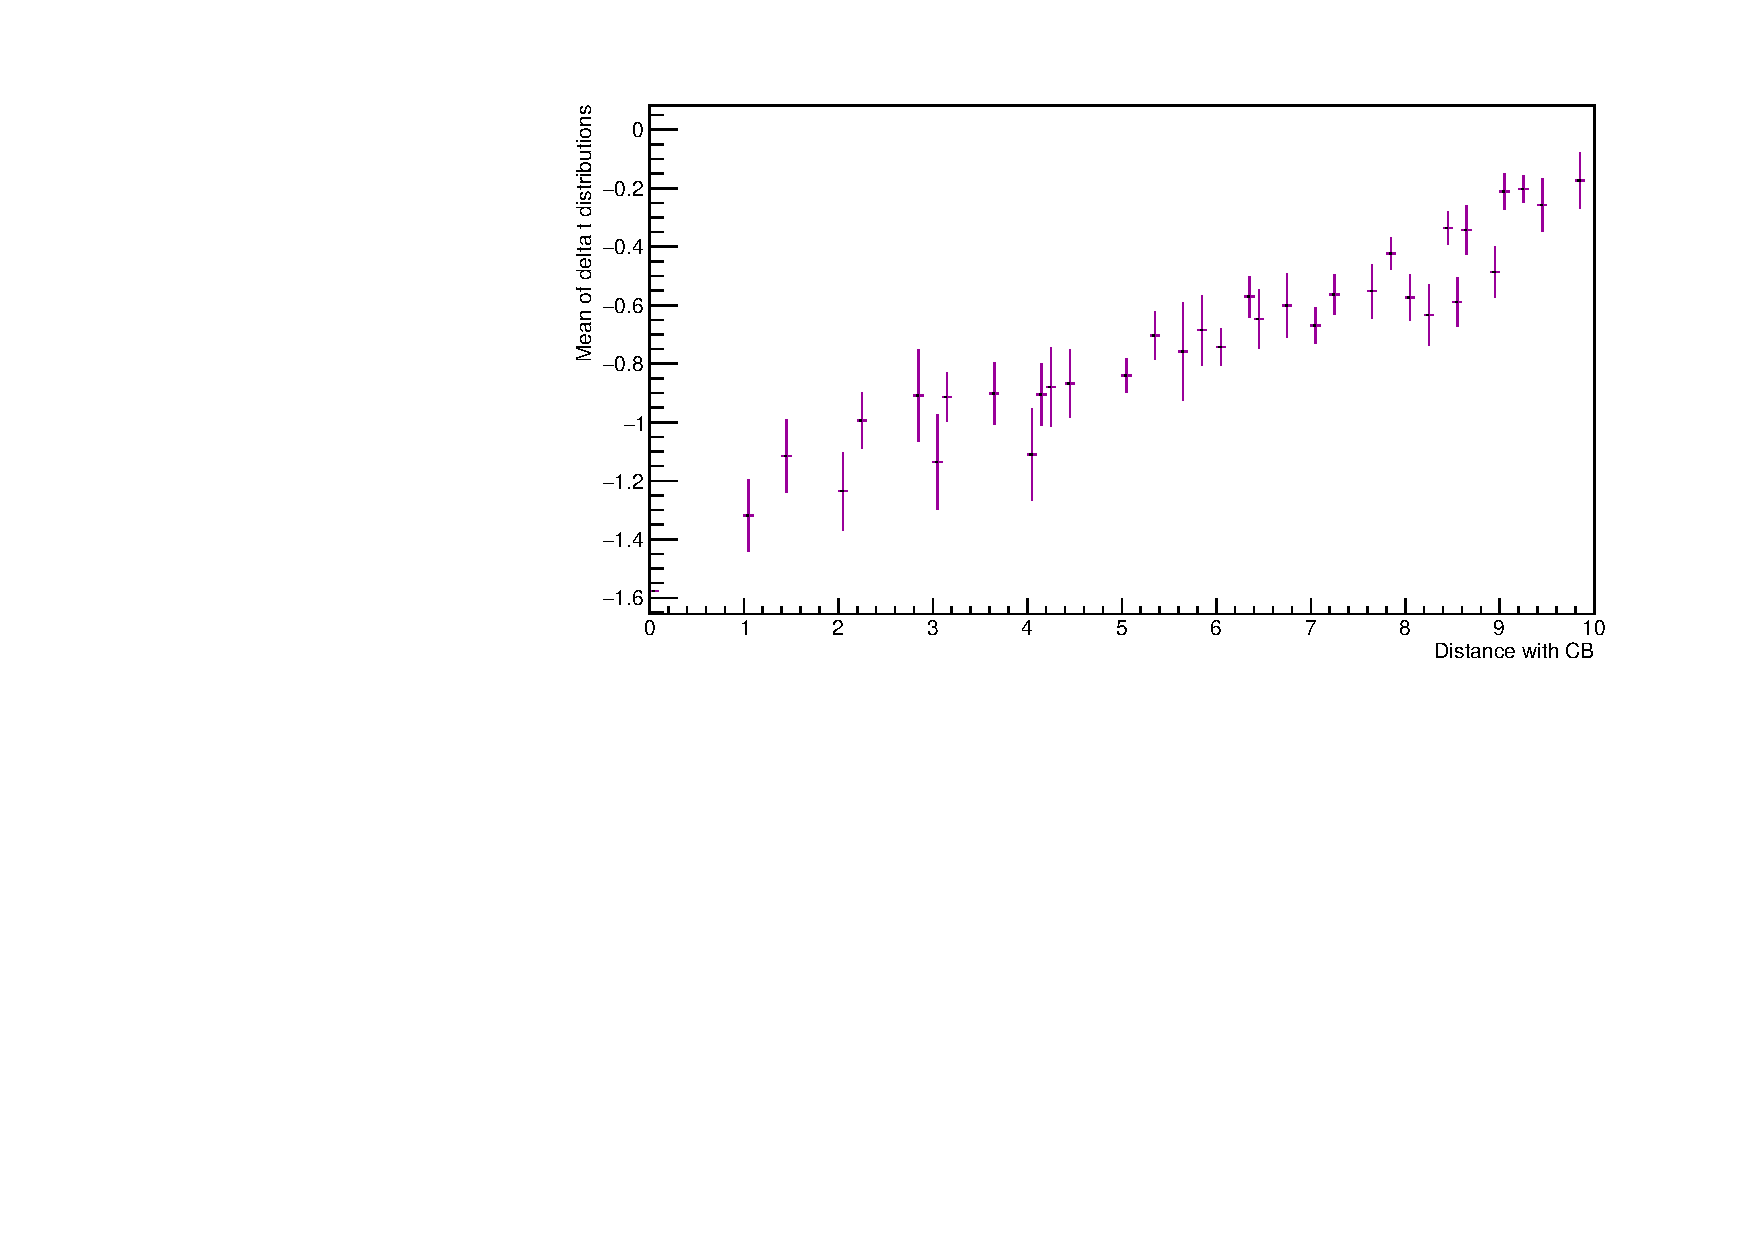
\includegraphics[width=0.9\textwidth]{commissioning/fig_commissioning/mean_distance.pdf}
  \caption{$\Delta t$ distribution mean as a function of the distance of the corresponding FEB with CB.
    \label{fig:mean_distance}}
\end{figure}

More than $800$ channels were calibrated: $3$ crates, $20$ FEBs for the two firsts and $12$ for the last one, each having $16$ electronic channels.
All time offsets have been stored in a database and made available for the collaboration.

%% \subsection{Comparison with $^{60}$Co}



%% \subsection{Principle}
%% \subsection{Measuring the time offset of front end boards}
%% \subsection{Results}


\section{Conclusion}

On this early autotumn $2020$, the calorimeter commissioning is almost complete, and a huge effort have been provided by the whole collaboration to calibrate it.
Automated codes have been developed to monitor changes in calorimeter characteristics over time (pulse shape, baseline, optical modules gain...).
The reflectometry analysis allowed us to control and record the lengths of all coaxial cables installed on the SuperNEMO demonstrator at LSM, and gave information on the status of cable connections at the patch panel.
We also have understood the main results on measured cable lengths.
The signal time delay induced by coaxial cables and front-end boards have been characterised and made available in databases.
In a subsequent analysis, the entire calibration chain will have to be calibrated in time, from the optical modules to the FEBs, using for example the LIS system sending light pulses in each scintillator.

All the work done to calibrate the calorimeter, and especially its time calibration, opens the door to the first physical data acquisition with the calorimeter.
Coincidence measurements of particle time-of-flights are therefore made possible by the characterisation of the time delay specific to each channel.
In the following chapter, we describe an experiment carried out with a \Co\ source to determine the time resolution of the optical modules, which follows the work presented in Chapter~\ref{ch:timediff}.
